%!TEX root = ../thesis.tex
\chapter{The Pleiades as a benchmark}
\label{chap:pleiades}

\section{Generalities}
\label{sect:generalities}
The ancient greeks named Pleiades to a crowded group of nine stars which they believed shared a common origin. These stars were the seven sisters, that together with their parents the titan Atlas and the nymph Pleione, were put in the sky  by the god Zeus.
 
Today, we call the Pleiades cluster not just to the nine stars that made up the original Pleione family, but to a much larger group, which according to \citet{Bouy2015} adds up to $\sim2100$ members. This cluster is fairly close to the sun, $\sim 134$ pc \cite[with parallaxes of $7.44\pm0.08$ and $7.48\pm0.03$ according to][respectively]{Galli2017,2017A&A...601A..19G}, and is also young in galactic scales, with only $\sim125$ \gls{myr} \citep{Stauffer1998}. Since it is located in the solar neighbourhood, it has a distinctive angular velocity in the plane of the sky: about $-16\,\mathrm{mas\cdot yr^{-1}}$ in right ascension and $20\,\mathrm{mas\cdot yr^{-1}}$ in declination. It has a metallicity near to the solar one \cite[{[Fe/H]$\sim$0},][]{Takeda2017}. Also, it has an almost null extinction of $A_v=0.12$ mag \citep{Guthrie1987}. These properties make the Pleiades one of the most studied clusters in the history of astronomy \footnote{Probably just after the Orion complex.}. Thus making it also the perfect test case of the methodology developed in this work.

As stated in the previous Chapter,  the objective of the present study is to obtain the statistical distributions of the distance, position, velocity, luminosity and mass of the Pleiades cluster. Thus, in the following sections I will describe the current knowledge of the Pleiades, concerning these astrophysical quantities. 
 
\section{The distance to the Pleiades}

\subsection{Measuring distances}
In astronomy, measuring distances is a complicated task. Techniques vary according to the distance scale that they aim to measure. The distance ladder is constructed from smaller to larger distances. The first step in this ladder is the distance to the sun. After that, the distance to the planets and then to the stars. This works deals only with nearby clusters, thus I only focus on measuring distances to these objects. 

The most direct way to measure distance to nearby stars is by means of the trigonometric parallax. This is the maximum relative angular displacement, with respect to the far distant stars, that an object suffers in the course of a year. {It is usually reported in miliarc seconds (mas)}. The relative displacement results from the movement of the Earth (thus of the observer) on its orbit around the sun. The relative displacement is maximal when measurements are taken at opposed points in the earth's orbit, when they are separated by six months. If the parallax were measured in seconds of arc and with infinite precision, then the distance to the object would be obtained by simply inverting its parallax. By doing so, the distance will be measured in parsecs. This unit gets its name from parallax-second. Thus an object located at a distance of one parsec from the sun shows a parallax of one arc second. The further the object is, the smaller the parallax gets.

As any measurement, parallaxes have uncertainties, which usually represent, or are a proxy for, the width of the distribution. {The parallax distribution is also continuous and non-limited}. 

When transforming parallaxes into distances we may be tempted to take a summary of the distribution, the mean for example, and just invert it to obtain the distance. This only holds if the summary corresponds to the true value (i.e. the statistic is unbiased). {The true value is that which would be observed in the presence of negligible uncertainties}. However, because measurements have uncertainties, which almost always are not negligible, the inversion of the parallax not always renders an unbiased estimate of the distance. {Assuming that the distribution of parallax measurements of an object is Gaussian, \citet{Lutz1973} found that the distance to the object can be reasonably recovered by just inverting the parallax if its relative uncertainty is below 0.15-0.20. However, the shape of the distribution of parallax measurements of an object (the second and higher order moments) plays also an important role. Transforming the parallax distribution into that of the distance require more than a simple inversion.}  

Several authors have proposed different approaches to the problem of distance determination using parallaxes, see for example \citet{Lutz1973,2015PASP..127..994B,2016ApJ...832..137A,2016ApJ...833..119A}. The proper way, as \citet{2015PASP..127..994B} points out, consists of inferring the true distances given the observed parallaxes. For that, a prior on the distance must be established. The authors mentioned before describe three different kinds of priors and the methodology needed to infer the true distances. However, going into deeper detail is beyond the scope of this work.

Now, I focus on the particular case of the distance to the Pleiades. One of the first measurements of the Pleiades distance using parallaxes was done by \citet{1999A&A...341L..71V} using \emph{Hipparcos} data.{ Later, the same author \citep{2009A&A...497..209V} refined his analysis and obtained a value of $120\pm1.9$ pc. However, \citet{2000ApJ...533..938G} with parallax measurements of seven stars taken at the Allegheny Observatory, and later \citet{2005AJ....129.1616S} with the parallaxes of three stars measured with the Fine Guidance Sensors of the \emph{Hubble Space Telescope}, derived distances of $130.9\pm7.4$ pc and $134.6\pm3.1$ pc, respectively. Finally, \citet{2014Sci...345.1029M} using very long baseline radio interferometric parallaxes of three stars obtained a distance of $136.2\pm1.2$ pc.} There was a clear controversy between \emph{Hipparcos} data and other parallax measurements. The current data release of the \gls{tgas}, gives a distance to the Pleiades of $133.7\pm0.5$ pc \cite[from a parallax of $7.48\pm0.03$ mas][]{2017A&A...601A..19G}. This seems to indicate that the \emph{Hipparcos} parallaxes were somehow biased.

Our research group finds a distance to the Pleiades of $134.4^{+2.9}_{-2.8} $ pc (from a parallax of $7.44\pm0.08$ mas) \citep{Galli2017}, which is in good agreement with the one of \gls{tgas}. We found this distance using the kinematic parallaxes delivered by the moving cluster technique. This essentially exploits the fact that since clusters are bound, their members show a clear kinematic footprint: they seem to converge to a point in the sky \citep{1964IAUS...20...50B}. Using this point and the velocity of the members (proper motion and radial velocities) it is possible to derive individual parallaxes. Furthermore, these individual parallaxes show a distribution which results from the dispersion of the cluster members distances along the line of sight. Figures \ref{fig:parallaxPhillip} and \ref{fig:parallaxTGAS} show the distribution of parallaxes for the Pleiades candidate members according to \citet{Galli2017} and \citet{2017A&A...601A..19G}, respectively. As can be seen from these Figures, the results of both works agree on the mean of the parallax distribution. However, they recover different variances. This difference results from the discrepancy in the number of objects, 1210 in \citet{Galli2017} vs. 152 in \citet{2017A&A...601A..19G}, and in the selection function of the two surveys. The \gls{tgas} sample is limited to the bright objects ($V \sim 11.5$ mag), whereas the \gls{ddr2} includes the faint end of the distribution ($i\sim25$ mag). For these reasons, in the following I adopt the distance found by \citet{Galli2017}.

Nevertheless, the distance distribution {(measured uncertainties comprised)} is only the depth component of the space distribution of the cluster, the other two components are given by the projected spatial distribution. 

\begin{figure}[ht!]
    \centering
    \begin{subfigure}[t]{\textwidth}
    \centering
        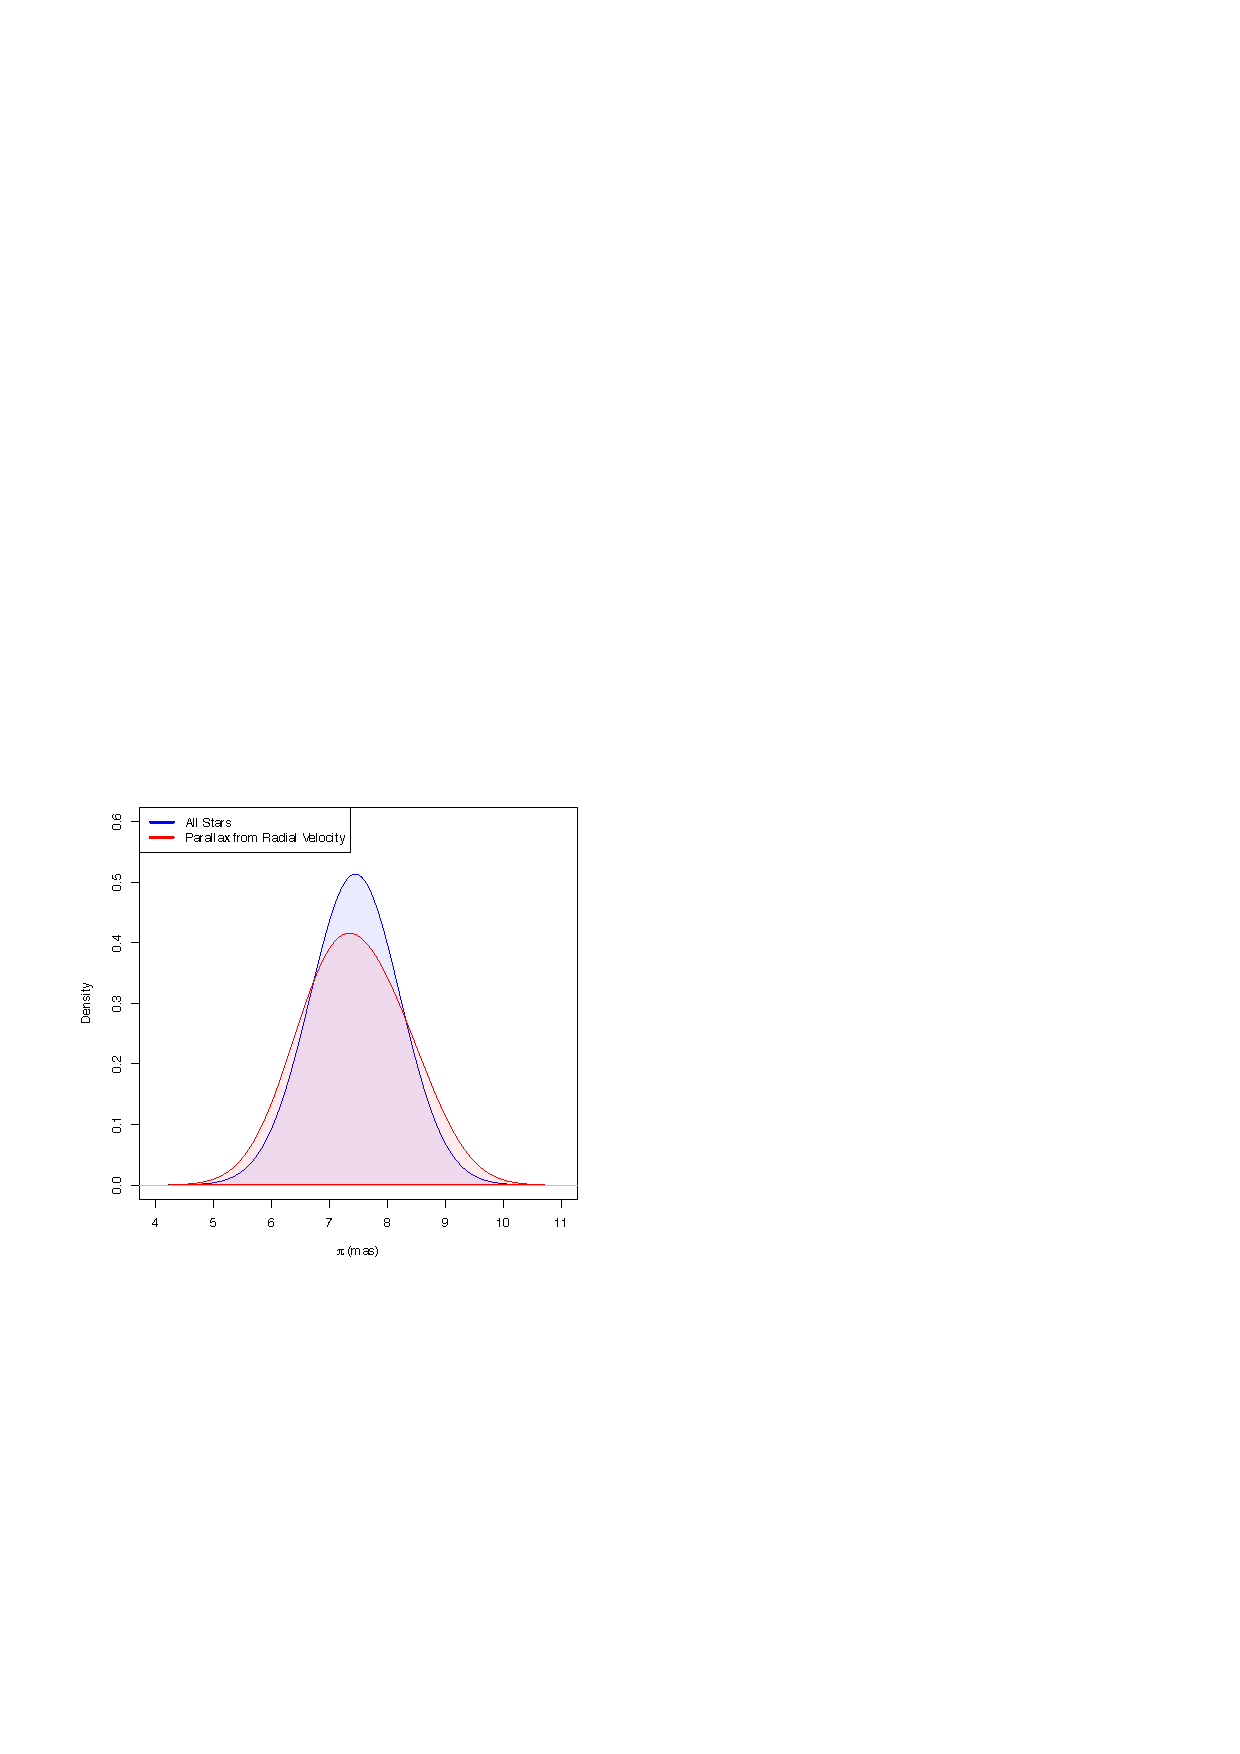
\includegraphics[height=8cm]{background/Figures/F13_Galli2017.pdf}
        \caption{Parallaxes according to \citet{Galli2017}. The red line shows all their candidate members (1210) while the blue one only those with known radial velocity (64). Reproduced from Figure 13 of \citet{Galli2017}, \textit{\usebibentry{Galli2017}{Title}}, \usebibentry{Galli2017}{Journal}, Vol. \usebibentry{Galli2017}{Volume}.}
        \label{fig:parallaxPhillip}
    \end{subfigure}
    \begin{subfigure}[t]{\textwidth}
    \centering
       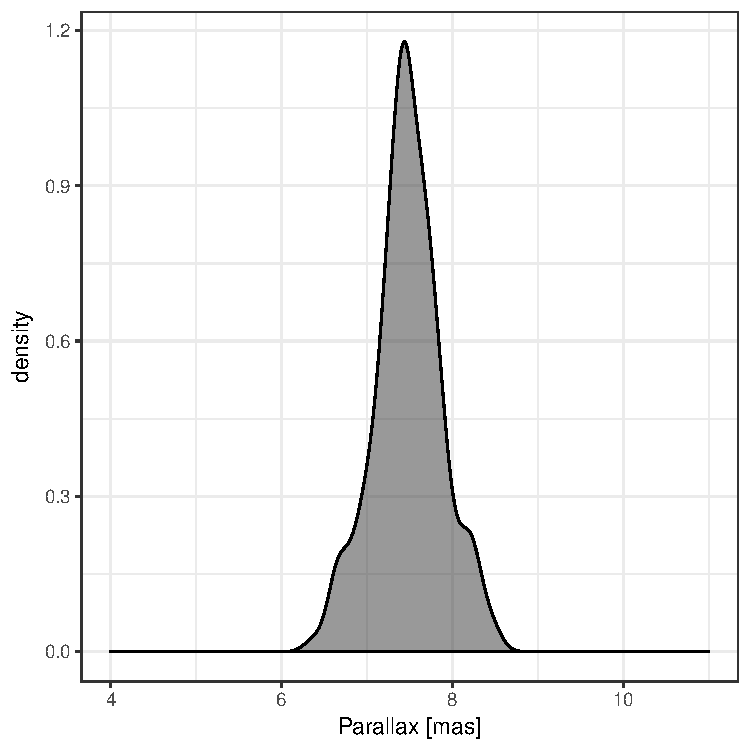
\includegraphics[height=8cm]{background/Figures/Parallax_GaiaCol2017.pdf}
        \caption{Parallaxes according to \citet{2017A&A...601A..19G}. Only their 152 candidate members.}
        \label{fig:parallaxTGAS} 
    \end{subfigure}
    \caption{Distribution of parallaxes for the Pleiades members.}
\end{figure}



\section{Projected spatial distribution}
\label{sect:PSD}
The \gls{psd} is the two dimensional projection, in the plane of the sky (the one perpendicular to the line of sight), of the cluster three dimensional space distribution. In astronomy, object positions are commonly measured in what is called the Equatorial Coordinate System\footnote{Another common coordinate system is the Alt-Azimuth one \cite[see][]{Smart1977}.}. It can be thought as the projection of the geographical coordinates, latitude and longitude, into the sky. The Right Ascension (R.A.) coordinate, analogous to the longitude, gives the objects angle with the vernal equinox, measured in an eastward direction and along the celestial equator. The Declination (Dec.) coordinate, analogous to the latitude, gives the object angle perpendicular to the celestial equator, positive to the North and negative to the South. For more details of the Equatorial Coordinate System see for example \citet{Smart1977}. 

{Stellar positions of an object are far more easily measured than its parallax. For this reason, just a small fraction of objects with stellar positions has also parallax measurements. In the case of the Pleiades, after cross-matching the \emph{Hipparcos} catalogue \citep{1997A&A...323L..49P} with the candidate members of \citet{Bouy2015}, I find that only 70 of the $\sim2100$ candidates have parallaxes. As seen in the previous section, this figure is roughly doubled with the new \gls{tgas} \citep{2016A&A...595A...1G} data release. In addition to the scarcity of parallaxes, which is expected to be solved with future \emph{Gaia} data releases, the relative uncertainties in R.A. and Dec. coordinates, measured in degrees, are far better ($\sim 10^{-5}$) than those of the parallaxes ($\sim10^{-1}$), measured in mas. Transforming these relative precisions into parsecs, by means of the distance, it is seen that the position in the plane of the sky is $10^4$ more precise than along the line of sight.  These two are the main reasons, for which the Pleiades space distribution has been studied mainly through its \gls{psd}. The latter has been the subject of several studies. }

One of the earliest results of the Pleiades \gls{psd} was done by \citet{Limber1962}. He used a mixture of four indices polytropic distribution, as was described is his earlier \citet{Limber1961} work, to fit the \gls{psd} of the 246 candidate members of \citet{Trumpler1921}. These candidates were contained in a $3^{\circ}$ radius around \emph{Alcyone} (one of the central most massive stars of the Pleiades cluster). 

\sloppy
Later, \citet{Pinfield1998} fitted King profiles \citep{King1962} to candidate members from the literature, which were contained in a $3^{\circ}$ radius area. They fitted King profiles to objects within different mass ranges, their bins centred at $5.2,1.65,0.83$ and $0.3 \,\mathrm{M_{\odot}}$. The tidal radius they found, $13.1\,pc$ ($\sim 5.6^{\circ}$) contained $1194$ candidate members. The total mass of these members amounted to $735\,\mathrm{M_{\odot}}$. These authors also estimated a mean individual stellar mass of $0.616\,\mathrm{M_{\odot}}$. {They measured core radius in the 0.9 to 2.91 pc range for the King profiles fitted to their different mass bins.}

On the same year \citet{Raboud1998} also fitted a King's profile \citep{King1962} to a list of 270 candidate members with masses in the range $0.74-7.04\,\mathrm{M_{\odot}}$, which were contained within a $5^{\circ}$ radius area. They found a core radius of $1.5$ pc and a tidal radius of $17.5$ pc ($7.5$ degrees). Using different approaches, they derived a total mass within the range of $500 -8000 \,\mathrm{M_{\odot}}$. They also measured an ellipticity of $\epsilon=0.17$, however they did not make any explicit mention on the position angle of the axis of the ellipse.

Later, \citet{Adams2001} also fitted a King profile to objects with membership probabilities $p>0.3$ within a radius of $10^{\circ}$. They found a core radius of $2.35-3.0$ pc and a tidal radius of $13.6-16$ pc ($5.8 - 6.8^{\circ}$). They estimate a total mass of $\sim 800\,\mathrm{M_{\odot}}$, and their measured ellipticities are in the range $0.1-0.35$. 

\citet{Converse2008} fit a King profile to a sample of 1245 candidate members from \citet{Stauffer2007} compilation. These objects have masses greater than $0.08\,\mathrm{M_{\odot}}$ and are contained within a $5^{\circ}$ radius. They obtained a tidal radius of $18$ pc (7.7 degrees) and a core radius of  $1.3$ pc. Later, \citet{Converse2010} refined their study and obtained a core radius of $2.0\pm0.1$ pc, a tidal radius of $19.5 \pm 1.0 $ pc ($\sim 8.3$ degrees) and a total mass of $870\pm35\,\mathrm{M_{\odot}}$. In Fig. \ref{fig:spatialConverse}, I reproduce the surface density fit obtained by these authors.

The previous summary of results shows at least two interesting points. In the first place, King profile \citep{King1962} has been the preferred choice for the Pleiades cluster, although it was created to fit the \gls{psd} of globular clusters. Since globular clusters are farther away than open clusters and in a low density environment, usually the end of their \gls{psd} is well within the survey area. The second point concerns the increasing trend of the tidal radius with the size of the survey and the publication date, see Table \ref{tab:tidal_iterature}. As the surveys increase in area the derived tidal radii increase as well. The exception is the work of \citet{Adams2001}. Since these authors used low membership probability ($\geq0.3$) objects, they may have also fitted the field. The surface density of a tidally truncated cluster should diminish with radius and eventually go to zero at the tidal radius. However, as can be seen in Figure \ref{fig:spatialAdams}, where I reproduce Figure 8 of \citet{Adams2001}, their surface density remains almost constant after $5^{\circ}$. This may be an indication of contamination in their sample. Furthermore, as those authors mention, they expect that the contamination dominates their sample outside the $5^{\circ}$ radius.

The two points mentioned before are tightly related. With the exception of the work of \citet{Adams2001}, the coverages of the rest of the surveys have not reached their estimated tidal radius. It indicates that the sample of members we currently have is spatially biased. It only contains objects from the inner parts of the cluster. Thus, estimates of the tidal radius may also biased. Nevertheless, this issue will be addressed with the full sky coverage of \emph{Gaia's} data.

\begin{figure}[ht!]
    \centering
    \begin{subfigure}[t]{0.49\textwidth} \centering
        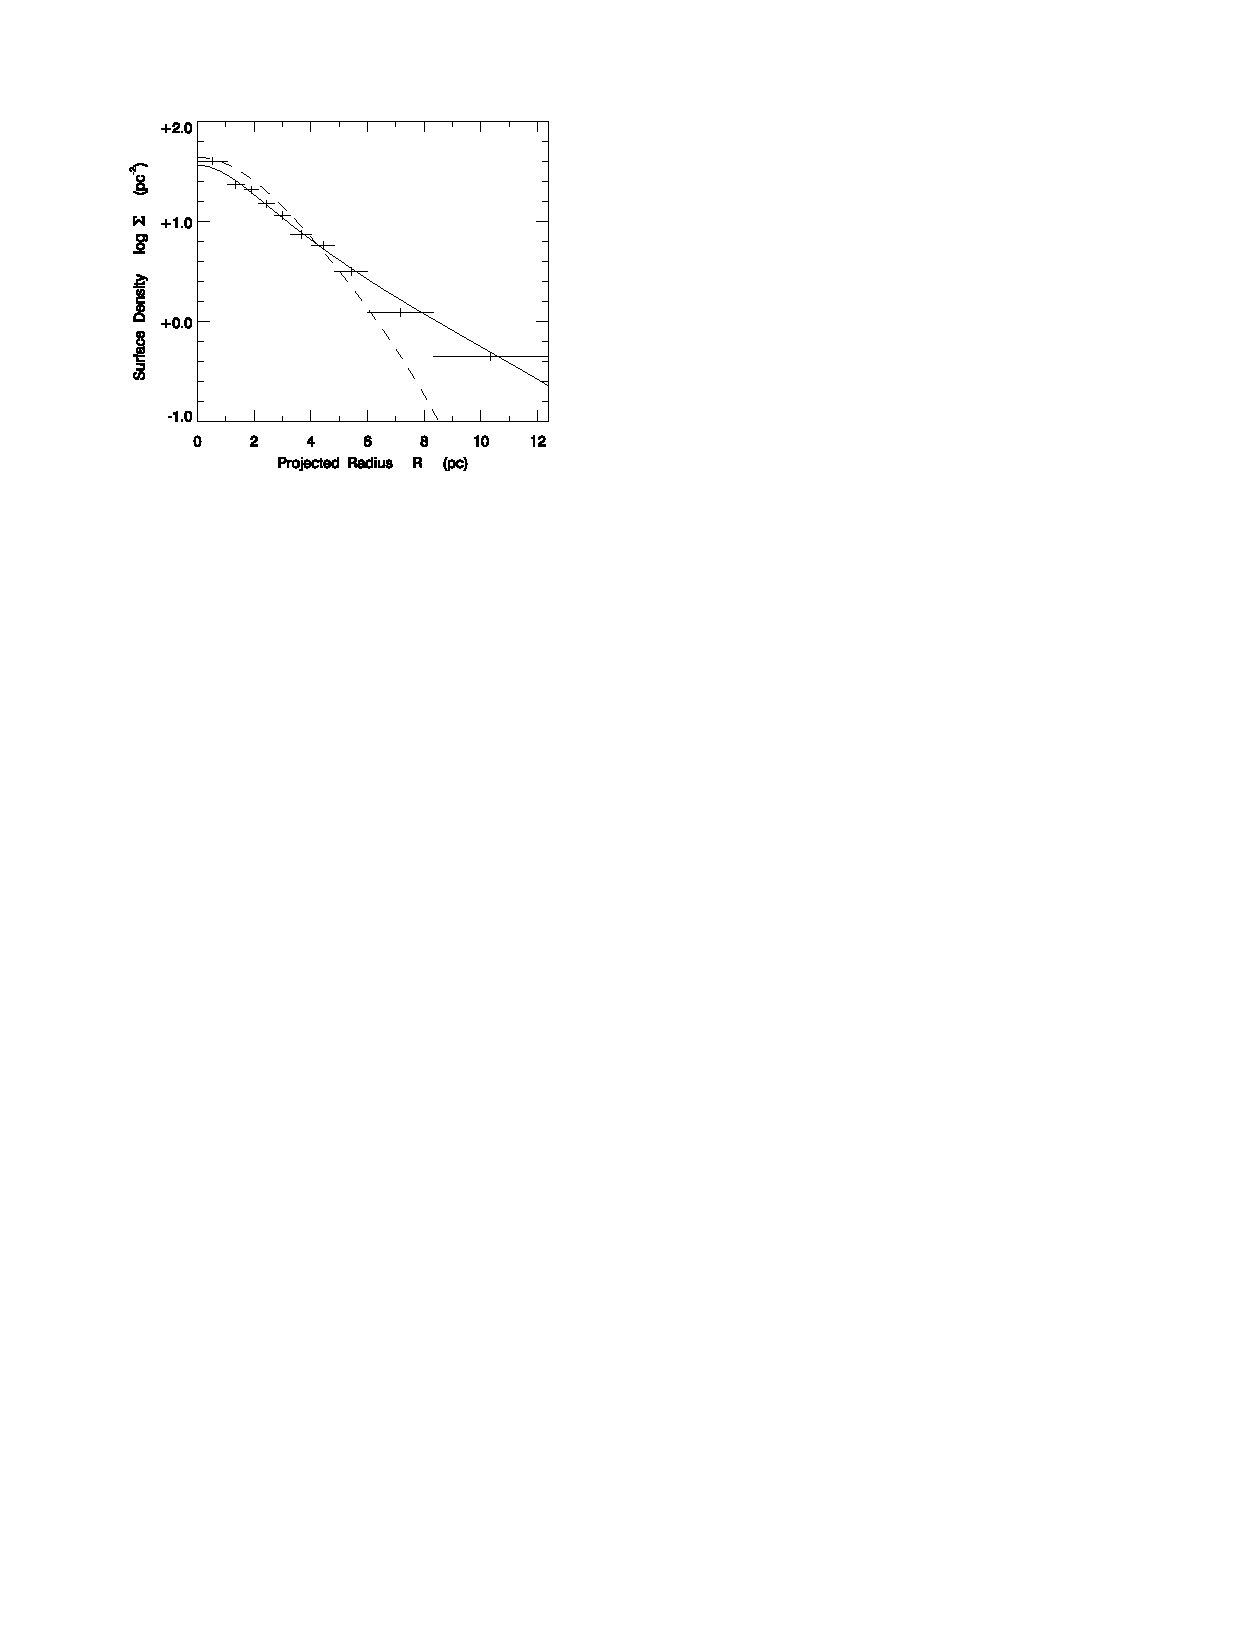
\includegraphics[height=6cm]{background/Figures/F1_Converse2010.pdf}
        \caption{}
        \label{fig:spatialConverse}
    \end{subfigure}
    \begin{subfigure}[t]{0.49\textwidth} \centering
       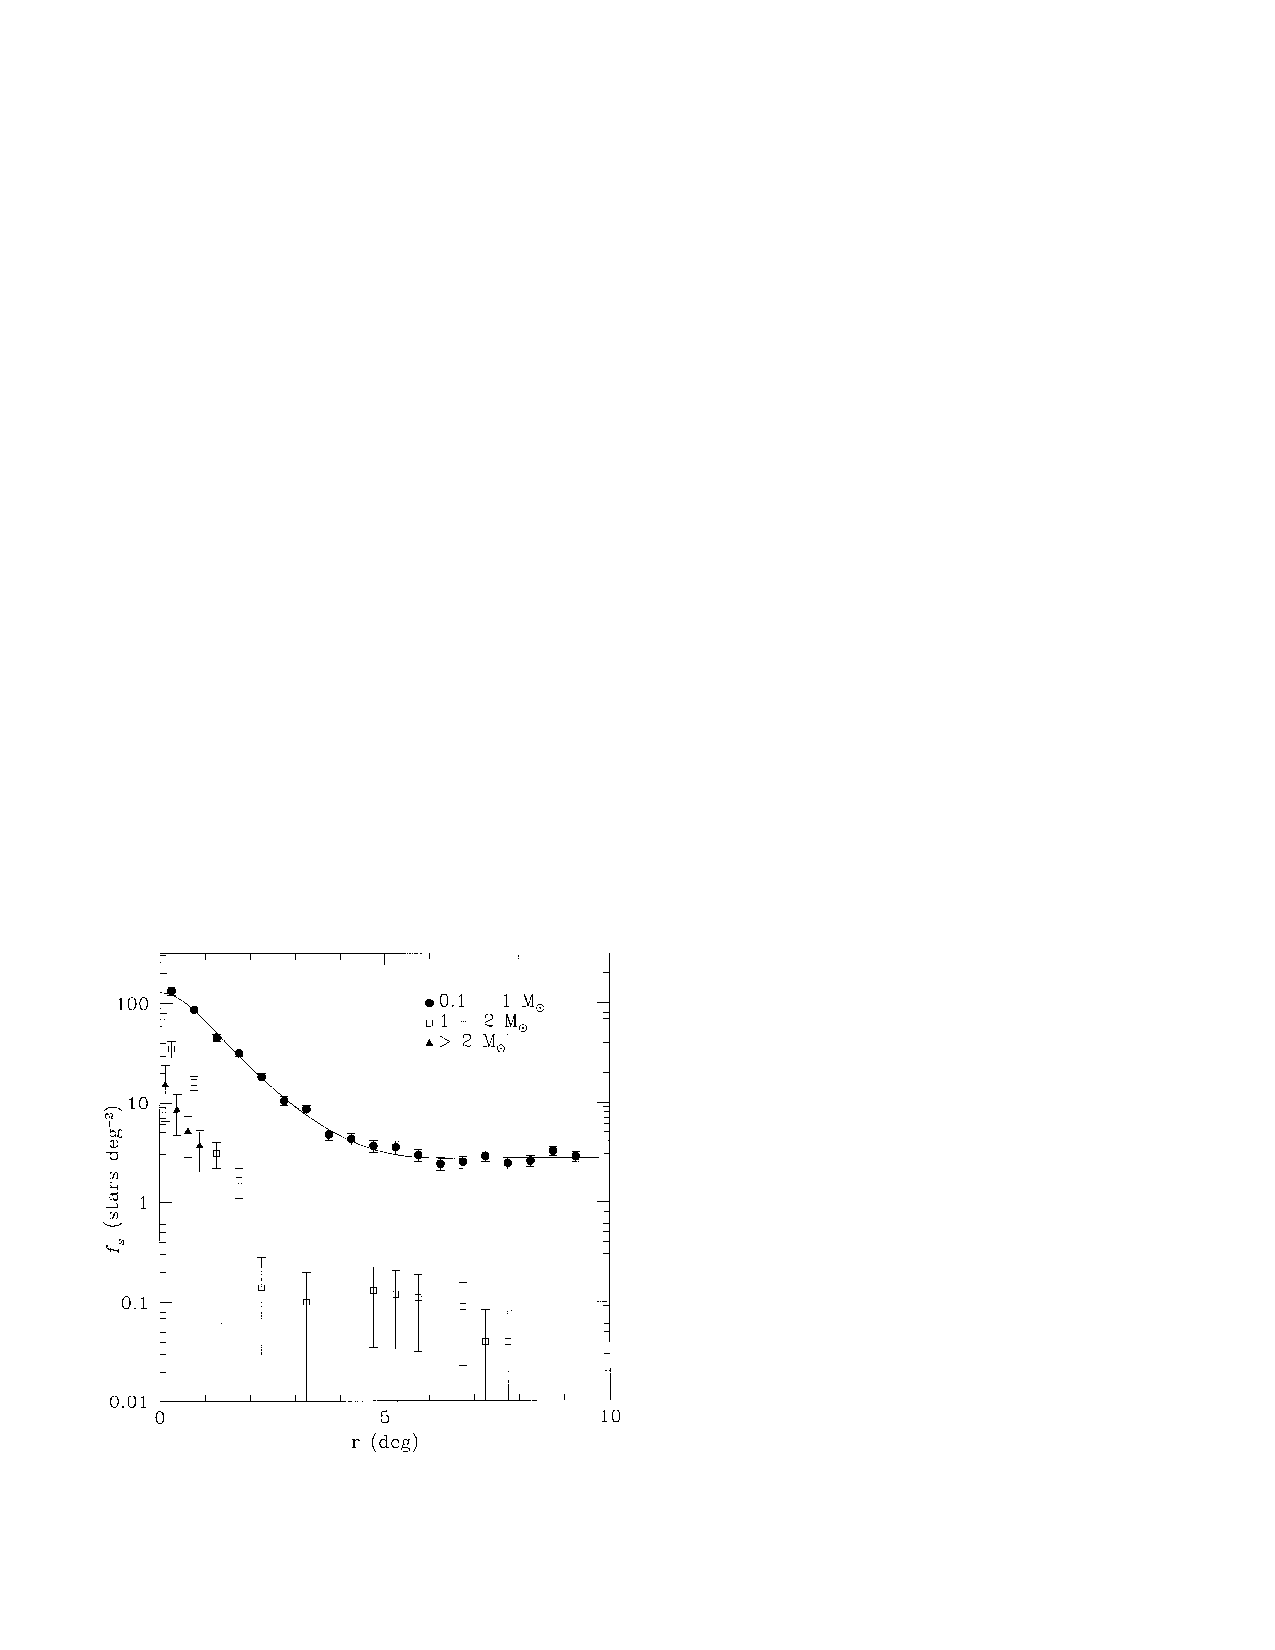
\includegraphics[height=6cm]{background/Figures/F8_Adams2001.pdf}
        \caption{}
        \label{fig:spatialAdams} 
    \end{subfigure}
    \caption{Projected spatial distribution of the Pleiades cluster. (a) Results from  \citet{Converse2010}. The crosses, and the dashed and solid lines represent the data and the fitted polytrope and King profile, respectively. Reproduced from Figure 1 of \citet{Converse2010}, \textit{\usebibentry{Converse2010}{Title}}, \usebibentry{Converse2010}{Journal}, Vol. \usebibentry{Converse2010}{Volume}. (b) Results from \citet{Adams2001}. The line shows the fitted King profile while the symbols are for different mass bins used. Reproduced from Figure 8 of \citet{Adams2001}, \textit{\usebibentry{Adams2001}{Title}}, \usebibentry{Adams2001}{Journal}, Vol. \usebibentry{Adams2001}{Volume}.}
\end{figure}

\begin{table}[ht!]
\caption{Survey, and derived core and tidal radius for recent studies in the literature. }
\begin{center}
\begin{tabular}{ccccc}
Authors &Core&Tidal& Tidal & Survey\\
&radius&radius&radius&radius\\
&(pc)&(pc)&($^\circ$)&($^\circ$)\\
\hline
\citet{Pinfield1998}&0.9-2.91&13.1&5.6&3\\
\citet{Raboud1998}&1.5&17.5&7.5&5\\
\citet{Adams2001}&2.35-3.0&16&6.8&10\\
\citet{Converse2008}&1.3&18&7.7&5\\
\citet{Converse2010}&2.0&19.5&8.3&5\\
\hline
\end{tabular}
\end{center}
\label{tab:tidal_iterature}
\end{table}%

  
\section{Velocity Distribution}

The three dimensional velocity distribution of the Pleiades has also been studied using its projections. One of them goes along the line of sight, it corresponds to the radial velocity. The other one is perpendicular to the previous one, lies in the plane of the sky, and corresponds to the transverse velocity. It is derived from  proper motions. These are angular velocities obtained after measuring the angular displacement of the object in at least two different epochs. Again, measuring the individual stellar position and its displacement over time is far easier than measuring radial velocities. These are measured using the Doppler shifted absorption lines in the spectre of the object. This shift is proportional to the object velocity relative to the observer along the line of sight. 

Since radial velocities require the object spectrum, their obtention for all cluster members, and particularly for the fainter ones, will demand a large amount of observing time. On the other hand, wide field images have been available for quite a long time, thus allowing long time base lines to measure proper motions.  Nevertheless, due to the Pleiades distance, radial velocities are often more precise than proper motion measurements, usually on the $1 \,\mathrm{km\cdot s^{-1}}$ regime. For these reasons, historically, the velocity distribution of the Pleiades cluster has been studied through the proper motions of its members. 

Probably the first description of the \gls{tvd} of the Pleiades is that of \citet{1884MNRAS..44..355P}. Using archival data from  Königsberg (1838-1841), Paris(1874) and Oxford (1878-1880) observatories, together with his own \emph{Differential Micrometer} observations, he was able to observe the relative displacements of 40 Pleiades stars. According to him \citep{1884MNRAS..44..355P}: \textit{the relative displacements of these distant suns, although not distinctly and accurately measurable in numerical extent, appear to vary both in direction and amount; indicating thereby the mutual influence of a group of gravitating bodies.} 

Later, \citet{Trumpler1921} used, for the first time, proper motion measurements to identify the members of the Pleiades cluster. He classified objects as candidate members according to the distance they show, in the proper motion space, to the mean proper motion of the cluster. This mean was previously calculated by Boss in his \emph{Preliminary General Catalog} \citep{1910pgcs.book.....B}. So far as my historic research went, Boss' work was the first measurement of a statistic of the \gls{tvd} of the Pleiades. 

Later \citet{1938AJ.....47...25T}, using Trumpler's data and archival compilations, was able to measure the dispersion of the proper motions distribution. He estimated it to be $0.79\,\mathrm{mas\cdot yr^{-1}}$($0.65\,\mathrm{ km\cdot s^{-1}}$ at 136 pc). This was probably, the first measurement of the second moment of the spatial velocity distribution. From this value he then derived a total mass of $260\,\mathrm{M_{\odot}}$.

In recent years \citet{Pinfield1998} used the velocity dispersion to probe that the cluster was in an state near to the virial equilibrium. Later, \citet{2006ARep...50..714L} used the projected radial and tangential velocity components of the spatial velocity distribution of 340 members to claim the absence of evidence for rotation, expansion or compression of the cluster. Also, he also found no evidence to support mass segregation. 

Concerning the radial velocities, the first record for the Pleiades correspond to \citet{1904ApJ....19..338A}. He measured the radial velocities of the six brightest stars. After this seminal work, more than a dozen of works have been published. Among them are the works of \citet{1924PhDT.........1W,1944ApJ...100..360S,1979BICDS..16....2M,1991ApJ...377..141L,1992A&A...255..130R,1994AJ....108..160S,1997A&A...320...74M,1996ApJ...469..706M,2000AJ....119.1303T,2006ARep...50..714L,2009AAS...21340702W,2009A&A...498..949M}, and \citet{2013AJ....146..134K}. In previous studies, the typical number of Pleiades candidate members was below 100 objects, with the works of \citet{2009AAS...21340702W} and \citet{2009A&A...498..949M} reaching 269 and 275 objects, respectively. The latest compilation of radial velocities from the literature is the one made made by \citet{Galli2017}. This list contains measurements for 394 objects. The distribution of these radial velocities is almost gaussian with a centre at $5.6\,\mathrm{km \cdot s^{-1}}$. In \citet{Galli2017}, we estimated a velocity dispersion of the $0.8\,\mathrm{ km\cdot s^{-1}}$ for the Pleiades candidate members.

Although, transverse and radial velocities are useful projections, the dynamical analysis of the cluster demands the three dimensional distribution. In \citet{Galli2017} we provide a list of 64 cluster members with full spatial velocities. The distributions of the three projections of these spatial velocities are shown in Figure \ref{fig:velocityGalli}.

\begin{figure}[ht!]
\begin{center}
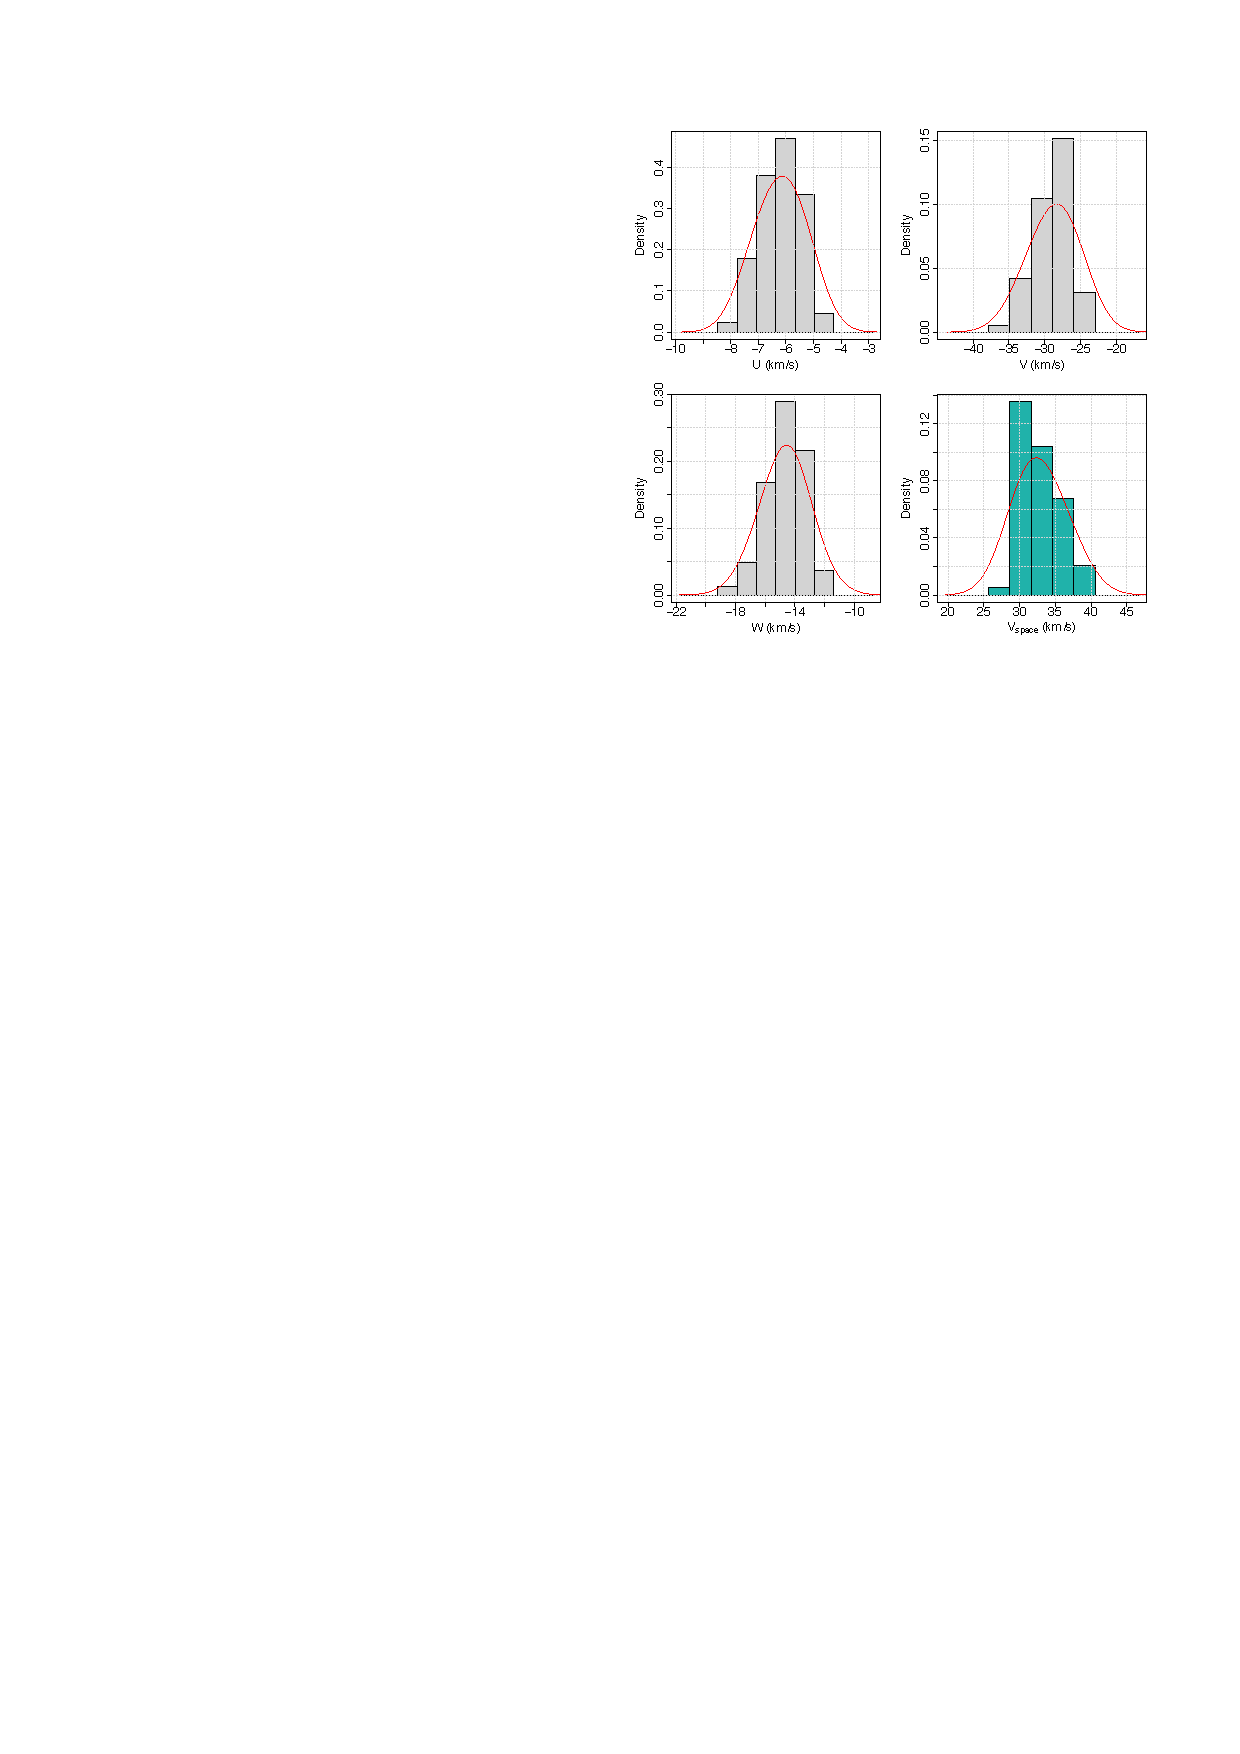
\includegraphics[width=0.8\textwidth]{background/Figures/F11_Galli2017.pdf}
\caption{Histogram and kernel density estimation (red line) of the components (grey) and modulus (green) of the spatial velocity distribution of 64 candidate members of \citet{Galli2017} with radial velocities and parallaxes. Reproduced from Figure 11 of \citet{Galli2017}, \textit{\usebibentry{Galli2017}{Title}}, \usebibentry{Galli2017}{Journal}, Vol. \usebibentry{Galli2017}{Volume}.}
\label{fig:velocityGalli}
\end{center}
\end{figure}

\section{Luminosity Distribution}

The luminosity distribution usually refers to the statistical probability distribution of the absolute\footnote{The absolute magnitude $M$, is the brightness that an object of apparent magnitude $m$ will show at a distance of 10 pc.} magnitude of the cluster population. It can also refer to the distribution of apparent magnitudes. It can be thought as the spectrum of brightness of the cluster members. Its importance lies in the fact the the luminosity of a star, measured in absolute magnitudes, can be related to its mass by the mass-luminosity relation. Therefore, the luminosity distribution is a proxy for the mass distribution. 

The study of the distribution of luminosities in the Pleiades started few years later than those of the positions and proper motions. The first record I found on the luminosity distribution is the one of \citet{Trumpler1921} (see Fig. \ref{fig:luminosityTrumpler}). He computed the number of stars in each magnitude bin for his two samples of candidate members, those comprising the objects within the central $1^{\circ}$, and those between $1^{\circ}$ and $3^{\circ}$, referred as Tables I and II, respectively. The completeness of the inner and outer samples was estimated at 14.5 and  9.8 photographic magnitudes (roughly 14 and 9 in the visual band), respectively. He observed that the luminosity distributions of these two samples were not alike, with the inner sample being brighter than the outer one. He also noticed that the luminosity distribution is not smooth, and shows a local minimum at 9 magnitudes, then an abrupt rise. Both effects are present in the two samples.

\begin{figure}[ht!]
\begin{center}
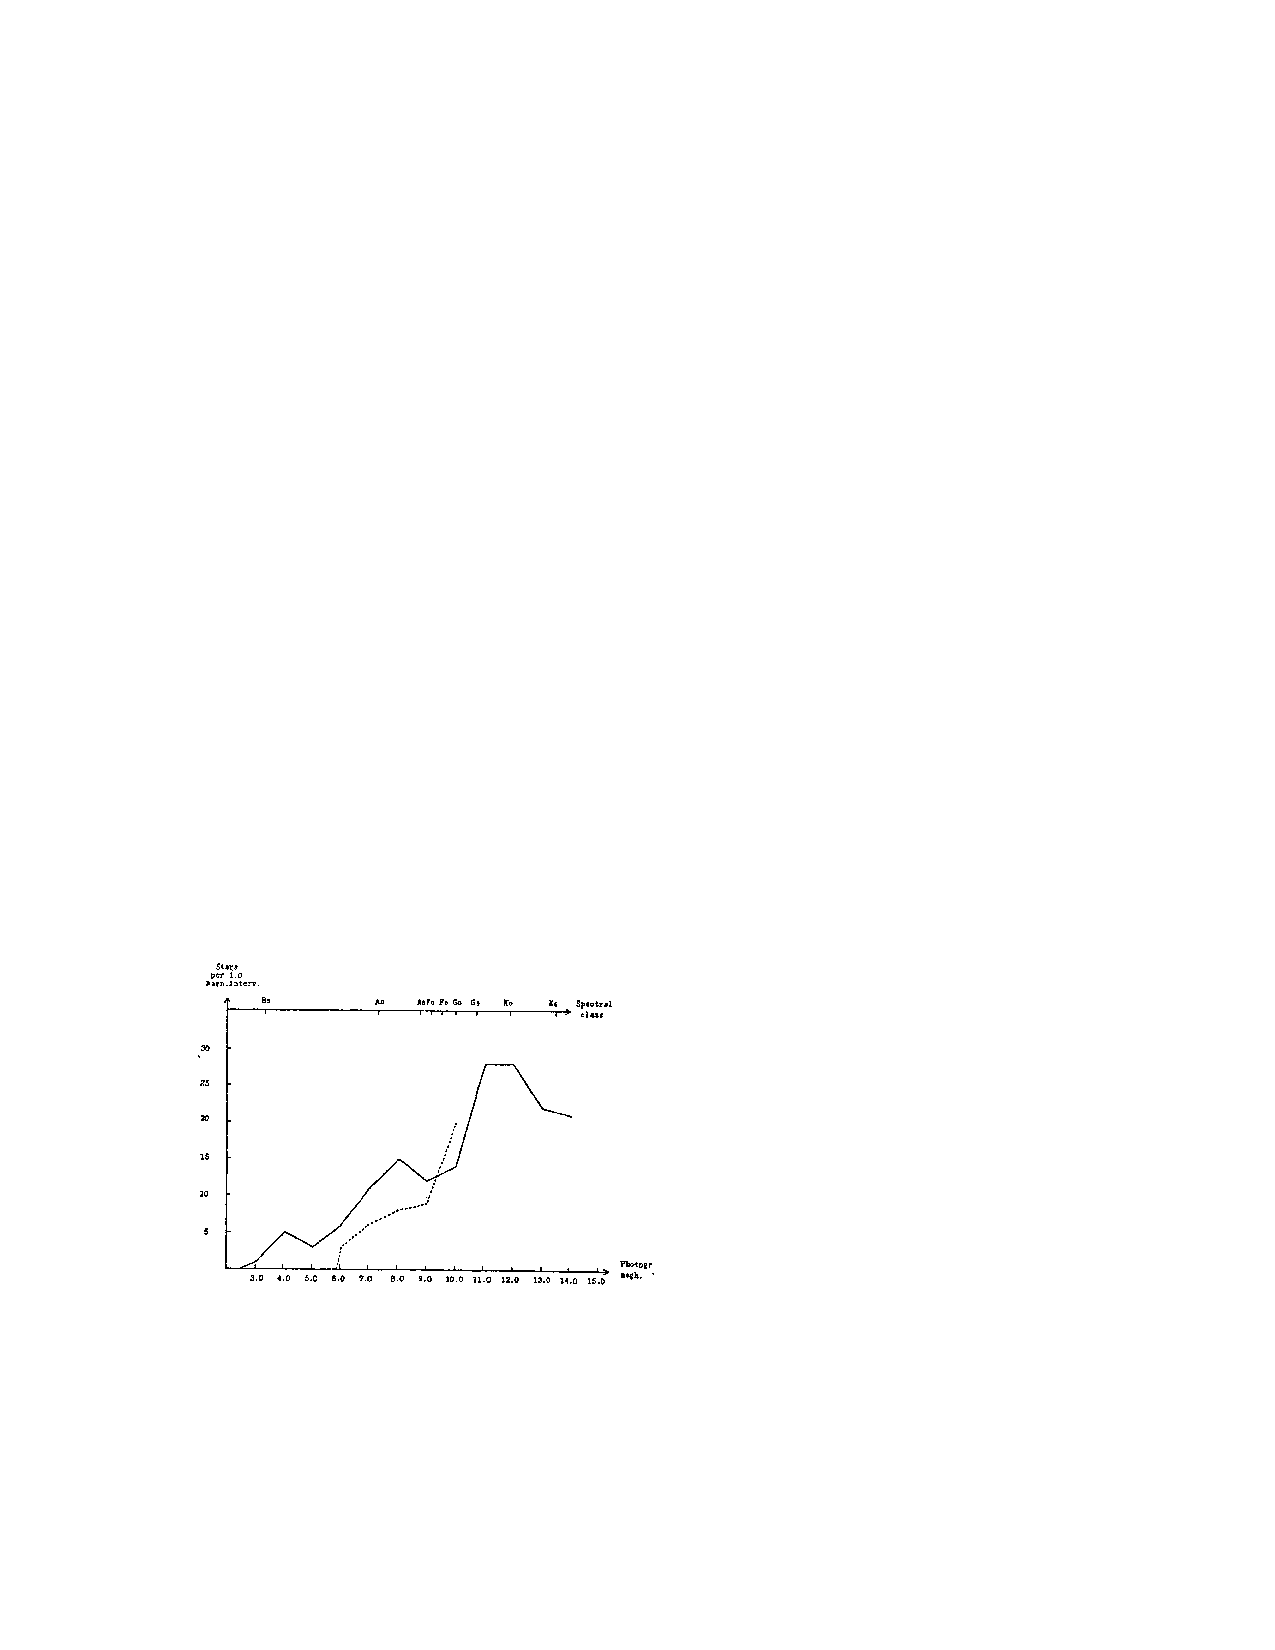
\includegraphics[width=\textwidth]{background/Figures/F2_Trumpler1921.pdf}
\caption{Luminosity distribution according to \citet{Trumpler1921}. The solid and dashed lines correspond to objects within $1^{\circ}$ and within $1^{\circ}$, and $3^{\circ}$ from the centre. Reproduced from Figure 2 of \citet{Trumpler1921}, \textit{\usebibentry{Trumpler1921}{Title}}, \usebibentry{Trumpler1921}{Journal}, Vol. \usebibentry{Trumpler1921}{Volume}.}
\label{fig:luminosityTrumpler}
\end{center}
\end{figure}

Later, \citet{Johnson1958} obtained the luminosity distribution using a sample of 289 candidate members. They assessed  membership solely on photometry. Their luminosity distribution is shown in Fig. \ref{fig:luminosityJohnson}

\begin{figure}[ht!]
\begin{center}
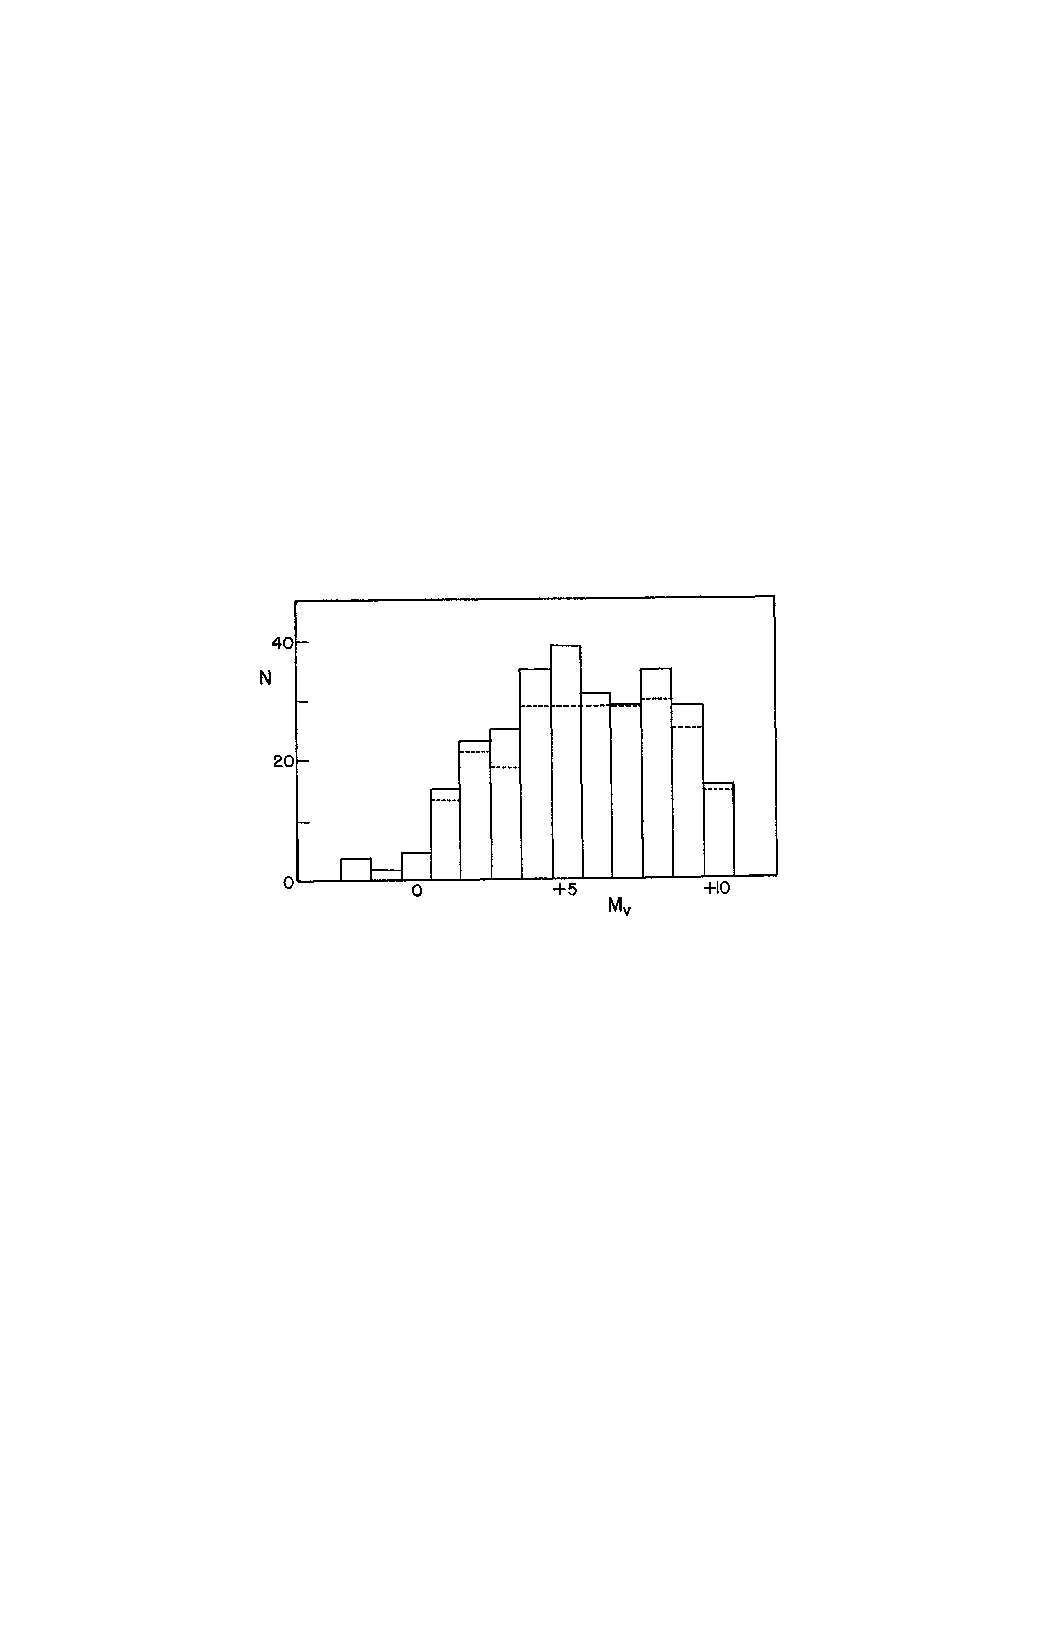
\includegraphics[height=8cm]{background/Figures/F3_Johnson1958.pdf}
\caption{Luminosity distribution in the visual band according to \citet{Johnson1958}. The dotted line represent the counts of main sequence stars only. Reproduced from Figure 3 of \citet{Johnson1958}, \textit{\usebibentry{Johnson1958}{Title}}, \usebibentry{Johnson1958}{Journal}, Vol. \usebibentry{Johnson1958}{Volume}.}
\label{fig:luminosityJohnson}
\end{center}
\end{figure}

Later, \citet{Limber1962} compared the luminosity distributions derived from the data of \citet{Trumpler1921}, \citet{Hertzsprung1947}, and \citet{Johnson1958}, with the initial luminosity distribution that he derived \citep{Limber1960}. The initial luminosity distribution corresponds to the distribution of luminosities that the cluster had at the moment of formation. \citet{Limber1960} derived it mixing data of galactic clusters and the local neighbourhood, and later correcting it by effects of age. He noted that the Pleiades present day luminosity distribution starts to differ from the initial luminosity distribution at visual magnitude $5.5$, see Fig. \ref{fig:luminosityLimber}. Assuming that this difference is due to the fact that stars fainter than $5.5$ have not yet had enough time for contraction, he derives an age of 50 \gls{myr}. 

\begin{figure}[ht!]
\begin{center}
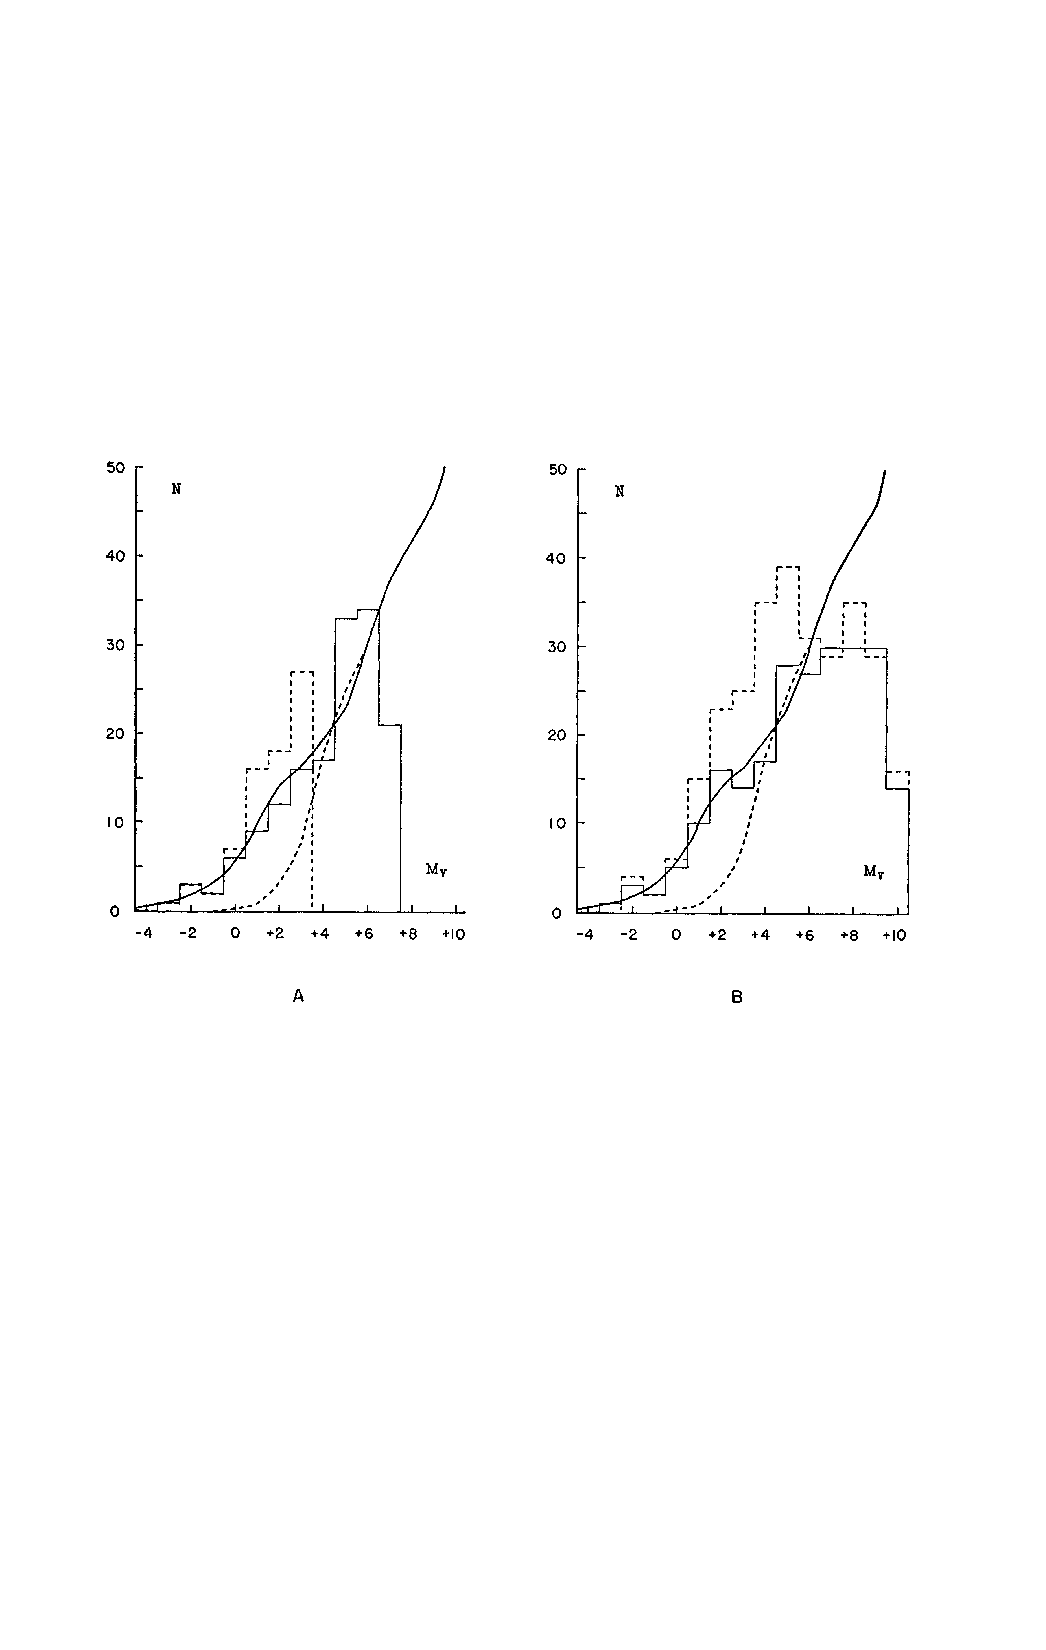
\includegraphics[height=8cm]{background/Figures/F4_Limber1962.pdf}
\caption{Luminosity distribution in the visual band according to \citet{Limber1962}.The solid and dashed histograms in: A correspond to \citet{Trumpler1921} data from the Tables II and I, respectively, in B, correspond to the data from \citet{Hertzsprung1947} and \citet{Johnson1958}, respectively. The solid and dashed curves line represent initial luminosity distribution and the present day luminosity distribution of the solar neighbourhood, respectively, both from \citet{Limber1960} . Reproduced from Figure 4 of \citet{Limber1962}, \textit{\usebibentry{Limber1962}{Title}}, \usebibentry{Limber1962}{Journal}, Vol. \usebibentry{Limber1962}{Volume}.}
\label{fig:luminosityLimber}
\end{center}
\end{figure}

In recent years, the luminosity distribution has been described in the works of \citet{Lodieu2012} and \citet{Bouy2015}. 
\citet{Lodieu2012}, using the \emph{UKIDSS} DR9 survey for galactic clusters and a probabilistic membership selection method (see discussion in Chapter \ref{chap:introduction}) based on proper motions only, and proper motions and photometry, found 8797 and 1147 candidate members, respectively. However, they do not provide the contamination rate in their analysis. Using both lists, they provide their luminosity distributions in the $Z$ band, which I show in Fig. \ref{fig:luminosityLodieu}.

\begin{figure}[ht!]
\begin{center}
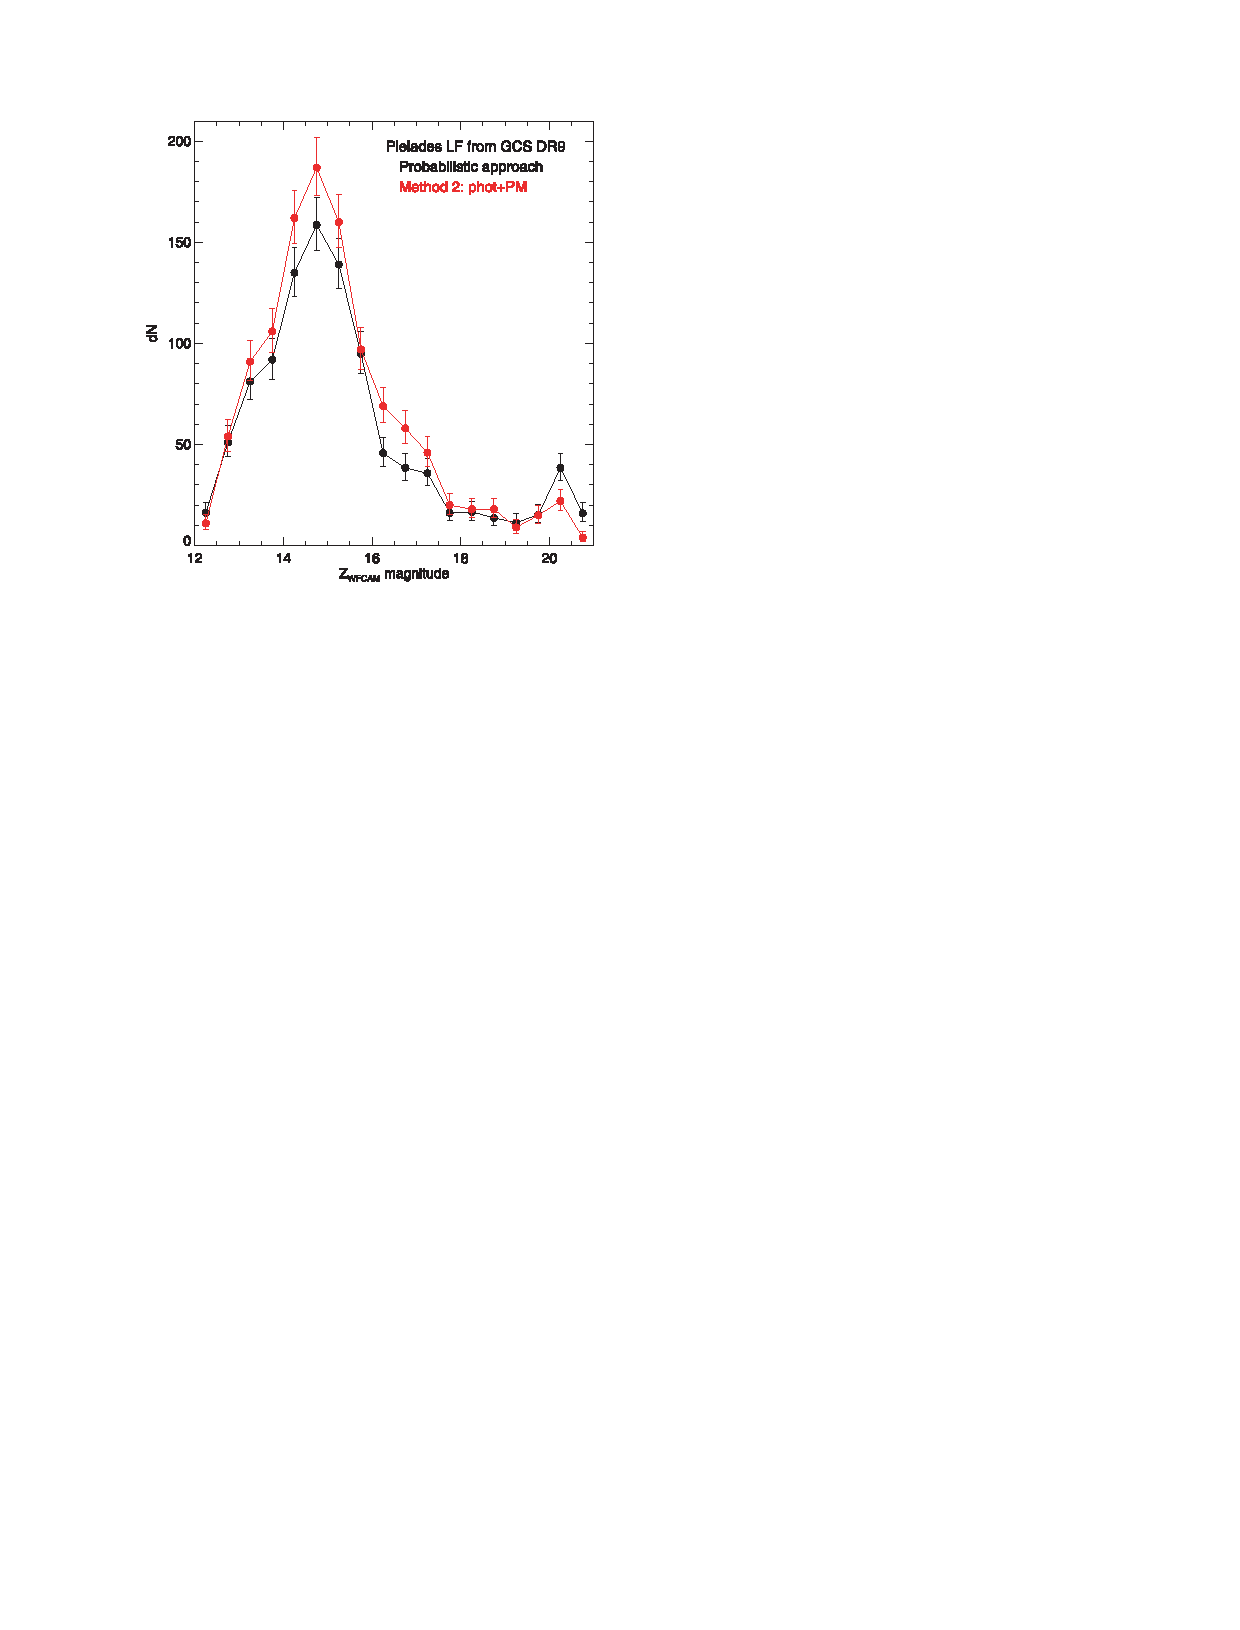
\includegraphics[height=8cm]{background/Figures/F9_Lodieu2012.pdf}
\caption{Luminosity distribution  in the $Z$ band according to \citet{Lodieu2012}. The red and black lines correspond to the two different probabilistic methods.  Reproduced from Figure 9 of \citet{Lodieu2012},\textit{\usebibentry{Lodieu2012}{Title}}, \usebibentry{Lodieu2012}{Journal}, Vol. \usebibentry{Lodieu2012}{Volume}.}
\label{fig:luminosityLodieu}
\end{center}
\end{figure}

In \citet{Bouy2015},  we estimated the present day system luminosity distribution of 1378 candidate members contained within the central $3^{\circ}$ region (with the centre at R.A.$=03:46:48$ and Dec.$=24:10:17$ J2000.0). It is called systemic because it has not been corrected for unresolved systems. An unresolved system is a group of stars (e.g. binaries) that due to its compactness appears as a single object. This distribution was computed for the $K_s$ band and is sensitive up to $K_s \sim 20$ mag and complete until $K_s \sim 17$ mag. This luminosity distribution is reproduced in Fig. \ref{fig:luminosityBouy}


\begin{figure}[ht!]
\begin{center}
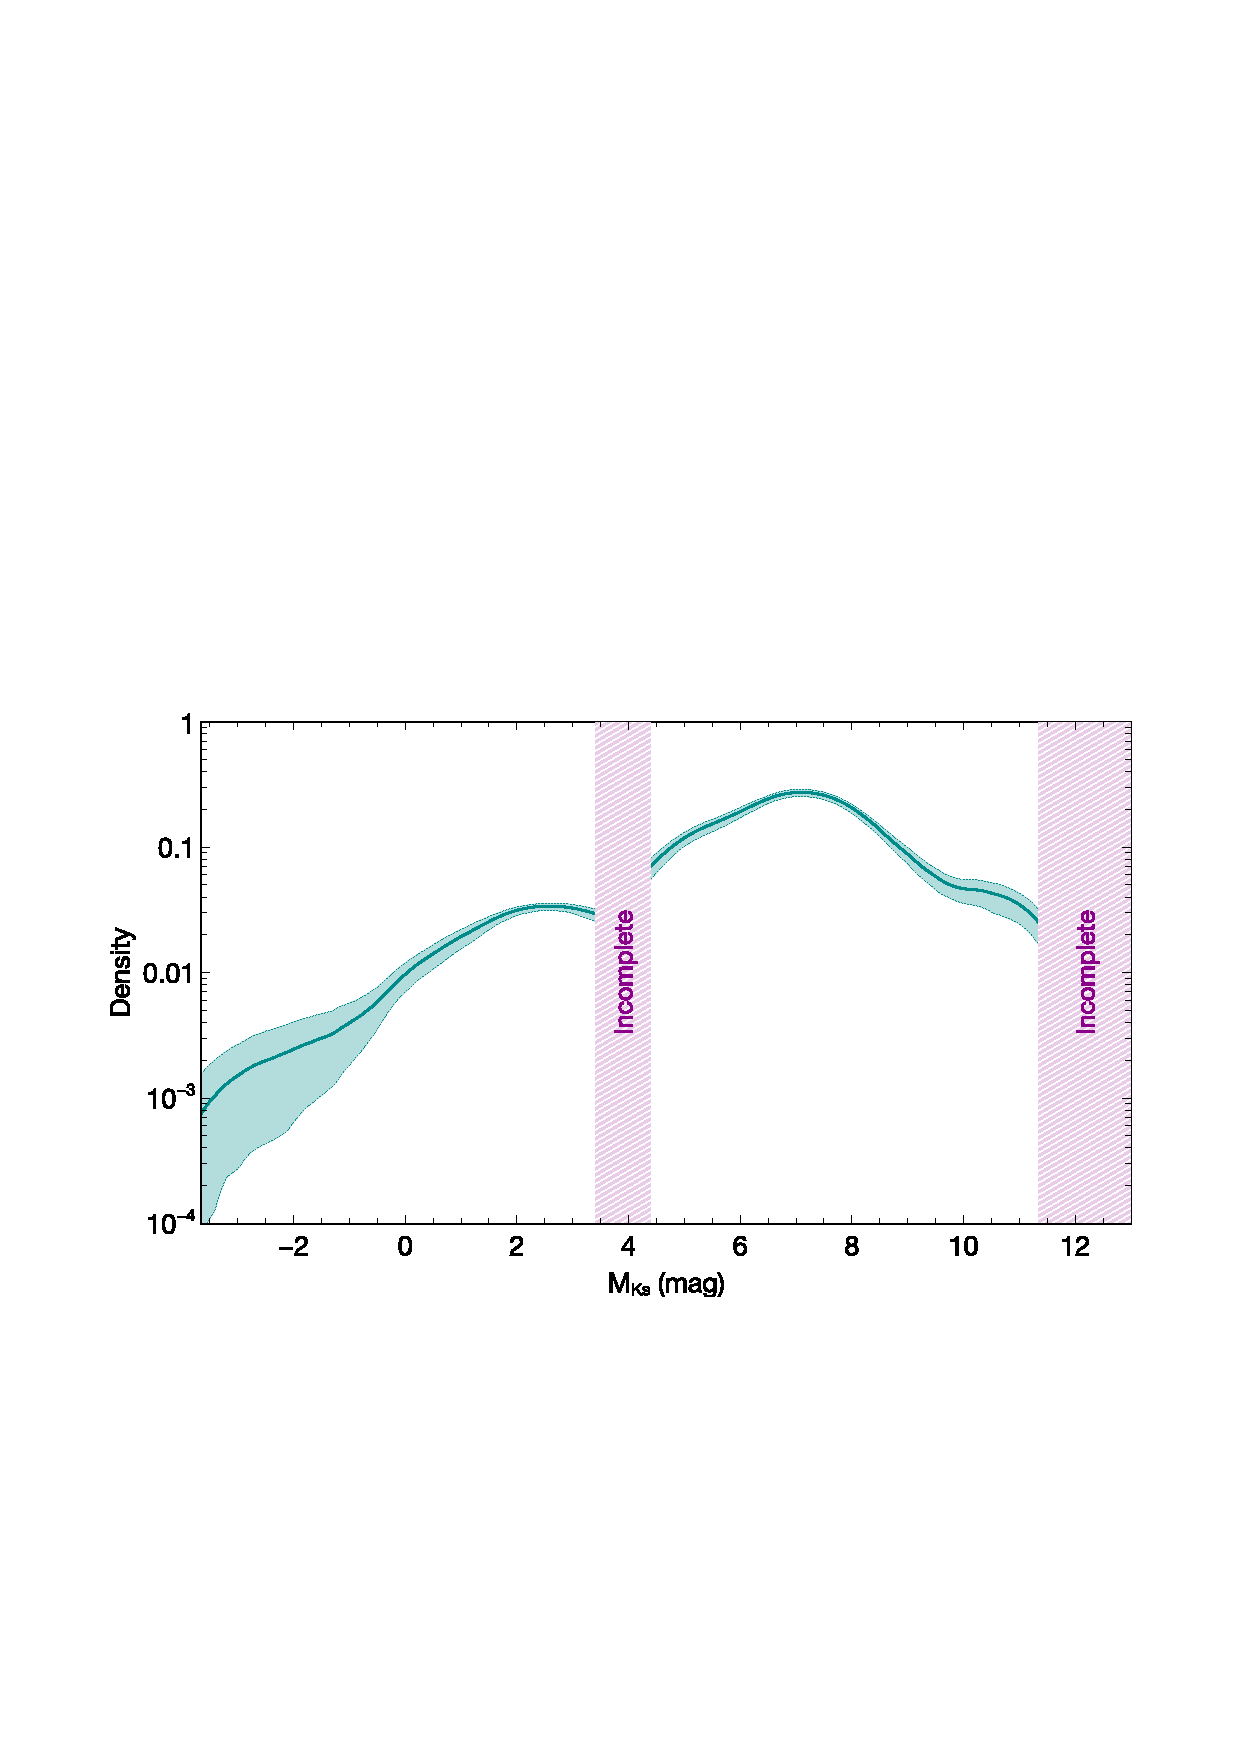
\includegraphics[width=\textwidth]{background/Figures/F8_Bouy2015.pdf}
\caption{Luminosity distribution in the $K_s$ band according to \citet{Bouy2015}. The incompleteness regions are shaded. Reproduced from Figure 8 of \citet{Bouy2015},\textit{\usebibentry{Bouy2015}{Title}}, \usebibentry{Bouy2015}{Journal}, Vol. \usebibentry{Bouy2015}{Volume}.}
\label{fig:luminosityBouy}
\end{center}
\end{figure}

\section{Mass Distribution}
\label{sect:mass}

In astrophysics, the mass distribution is a cornerstone in the understanding of the star formation process and the later evolution of stellar systems. Although the temporal evolution of these systems is mainly dominated by the gravitational potential, the initial conditions and an ongoing star formation process, if any, can contribute to the shape of the mass distribution. This last contains the fingerprints of past events in the history of the cluster and plays a key roll in its future evolution. Indeed, the evolution of the mass distribution is an essential element in one of modern astrophysics' objectives: the determination of the roll played by the initial conditions or the environment, in the temporal evolution of the stellar systems. The mass distribution at the moment of the cluster formation, which is known as the initial mass distribution evolves in time according to: i) stellar internal and atmospheric processes (e.g. contraction, mass loss, inflation, supernova events), ii) population dynamical interactions (e.g. three-body encounters, runaway stars, stellar evaporation), and iii) galactic dynamics (e.g. tidal effects, encounters with other clusters). For these reasons, the study of the initial mass function and its posterior evolution is a key element in the current understanding not just of open clusters but also of galactic and extragalactic populations.  


The mass distribution of the Pleiades has been largely studied. The first work on the mass distribution is that of \citet{Limber1962}. Although he did not show any graphical or tabular representation of it, he gave the luminosity distribution and the mass-luminosity ratio. Form these the mass distributions can be derived. Instead, he use them to obtain the total mass of the cluster ($760\,\mathrm{M_{\odot}}$, see next Section). 

Most probably, the first work to present the mass distribution derived from luminosity distributions and a mass-luminosity relation from theoretical models was that of \citet{Hambly1991}. Using $R$ and $I$ observations from the \emph{United Kingdom Schmidt Telescope Unit} together with the mass-luminosity relation from theoretical isochrone models of Padova group, he was able to transform his luminosity distribution into a mass distribution. In Fig. \ref{fig:massHambly}, I reproduce his results. 

\begin{figure}[ht!]
\begin{center}
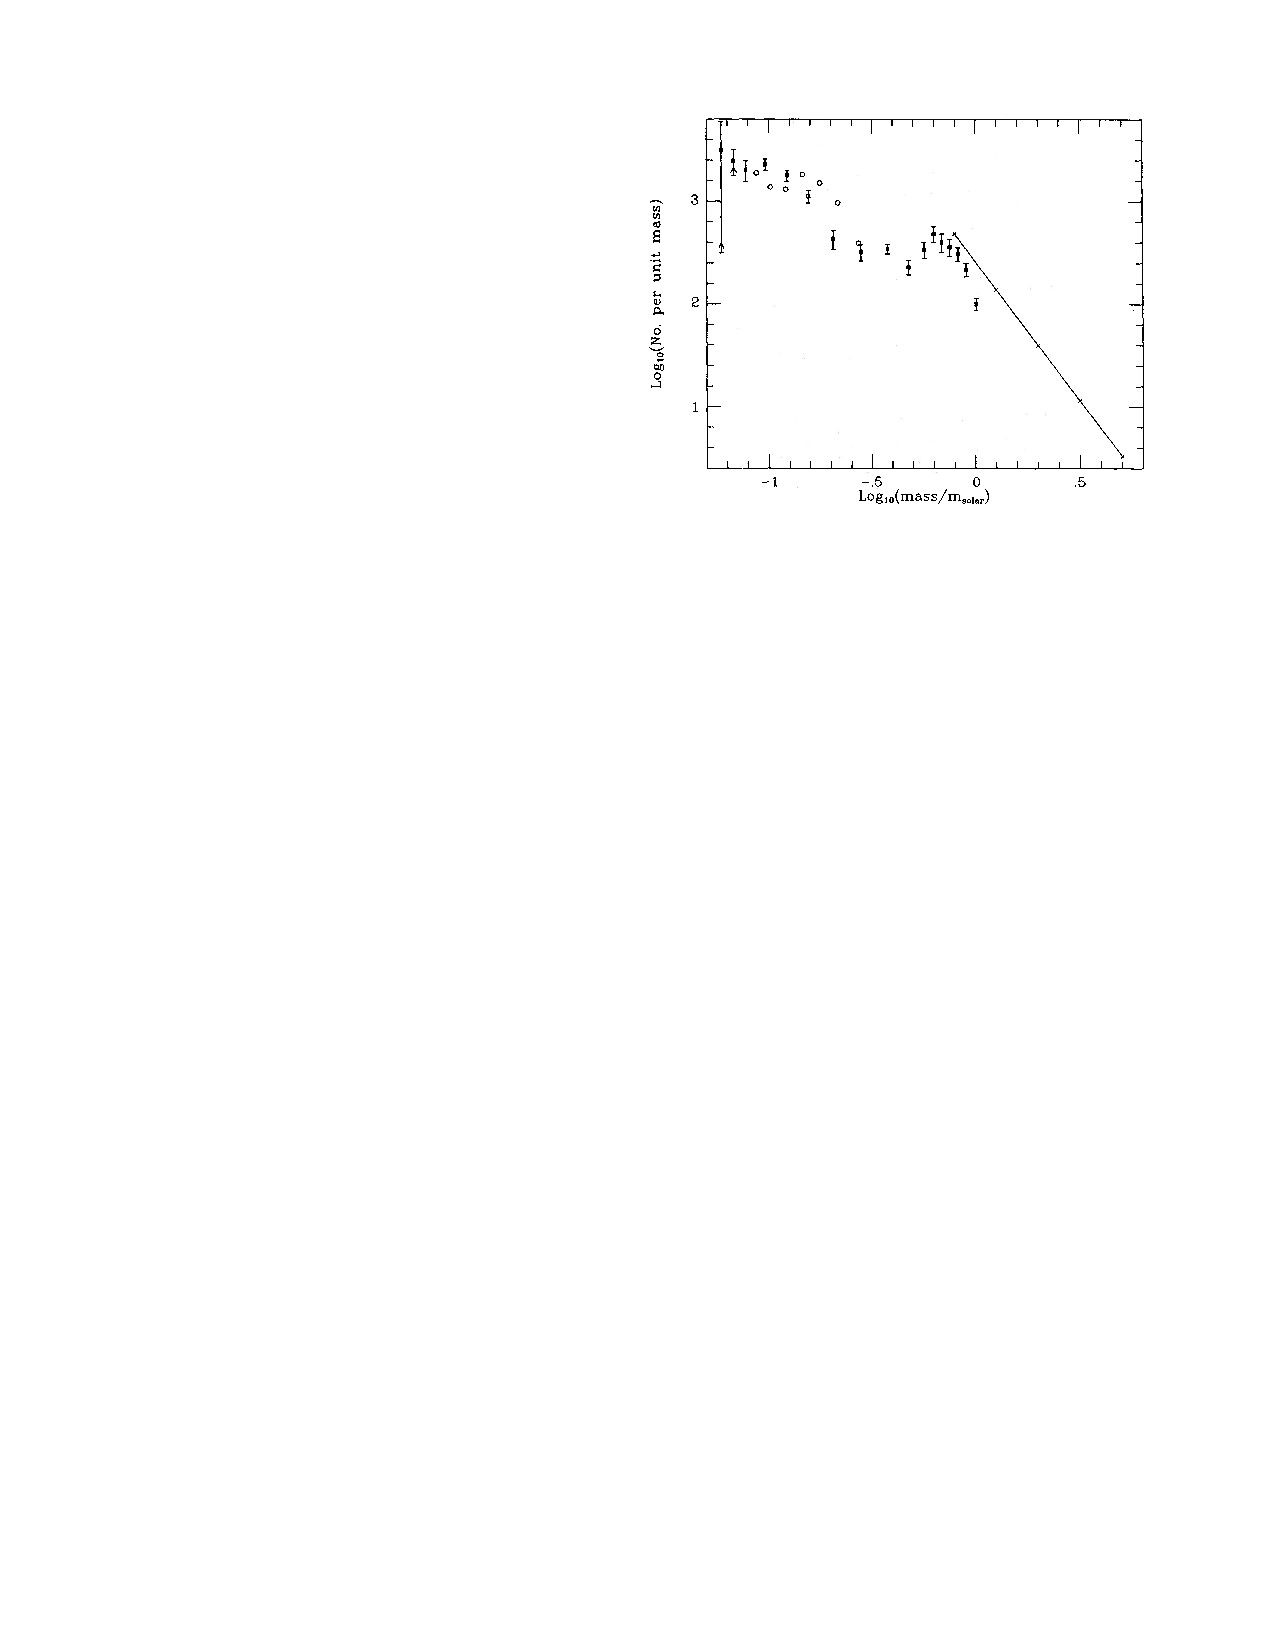
\includegraphics[height=8cm]{background/Figures/F11_Hambly1991.pdf}
\caption{Mass distribution of \citet{Hambly1991} derived from luminosity distribution and theoretical isochrone models. The open circles result from assuming an older age of 200 \gls{myr}. The line represent the mass distribution of \citet{1980IAUS...85..157V}. Reproduced from Figure 11 of \citet{Hambly1991},\textit{\usebibentry{Hambly1991}{Title}}, \usebibentry{Hambly1991}{Journal}, Vol. \usebibentry{Hambly1991}{Volume}.}
\label{fig:massHambly}
\end{center}
\end{figure}

From the year 2000 till date, several studies have been published in which the subject of analysis is the Pleiades mass distribution, e.g. \citet{2000ASPC..198...59H, 2002MNRAS.335..853J, 2001A&A...367..211M,2003A&A...400..891M, 2004A&A...426...75M, 2007MNRAS.380..712L}. However, for the sake of simplicity, here I only analyse the two most recent works, those of \citet{Lodieu2012} and \citet{Bouy2015}. The \gls{pdsmd} derived from both these works are shown in Figs. \ref{fig:massLodieu} and \ref{fig:massBouy}. These works obtained first the luminosity distribution, and then transformed it into a mass distributions using mass-luminosity relations of theoretical isochrone models. 

\citet{Lodieu2012} used a distance of 120.2 pc, an age of 120 \gls{myr}, and the \emph{NEXTGEN} theoretical models of \citet{1998A&A...337..403B} to transform the luminosity into the mass distribution. On the other hand, in \citet{Bouy2015} we use a distance of 136.2 pc an age of 120 \gls{myr} and the \emph{BT-Settl} theoretical isochrone models of \citet{2014IAUS..299..271A}. 

Both works found that their derived \gls{pdsmd} are in general agreement with the \gls{imf} of \citet{Chabrier2005} for unresolved systems (see Section \ref{sect:IMF}). However, in \citet{Bouy2015} we pointed out that, assuming that the theoretical mass-luminosity relation is correct, the \glspl{imf} of \citet{Chabrier2005} and \citet{Thies2007} predict too many low-mass stars and brown dwarfs in the range $0.04-0.1\,\mathrm{M_{\odot}}$. 

The differences at the low mass regime between the \gls{pdsmd} derived by \citet{Lodieu2012} and \citet{Bouy2015} (see Figs. \ref{fig:massLodieu} and \ref{fig:massBouy}) could arise from the different i) samples of members, ii) mass-luminosity relations, and iii) distances adopted by both works.

The different distances can introduce a general shift in the luminosity, which in turn can shift the mass distribution. This shift in luminosity, however, can be neglected due to its small value, $0.06$ mag.

Concerning the differences between the mass-luminosity relations of the two isochrone models, \citet{2013MmSAI..84.1053A} show that there are clear differences between the effective temperatures delivered by the \emph{BT-Settl} and the \emph{NEXTGEN} models in the low-mass regime, at $5$ Gyr particularly. {However, they do not discuss how this difference change in younger ages. Thus, this effect can not be discarded as the source of the differences.}

Concerning the differences between the lists of candidate members, \citet{Lodieu2012} do not provide (at least explicitly) any estimate of contamination rate of their samples. Furthermore, their membership methodology has some draw backs \cite[see][]{Sarro2014} that may have biased their results. {Therefore, the agreement that \citet{Lodieu2012} found between their present day mass distribution and the \gls{imf} of \citet{Chabrier2005}, which models the field mass distribution, may be an indication that their sample of candidate members is contaminated by the field.  }

On the other hand, in \citet{Bouy2015} we estimated a contamination rate of 7\%. However, we have no evidence for it to be non-homogeneous in mass. Even if the 7\% contaminants were not homogeneously distributed in the mass range, this value is not able to account for the observed discrepancies ($30-40\%$ in the low-mass regime) between the \gls{imf} of \citet{Chabrier2005} and our present day mass distribution.

The previous studies show that there is still work to do in the analysis of the Pleiades mass distribution, particularly at the low-mass regime where the \glspl{imf} show discrepancies with the observed present day mass distribution.  

\begin{figure}[ht!]
\begin{center}
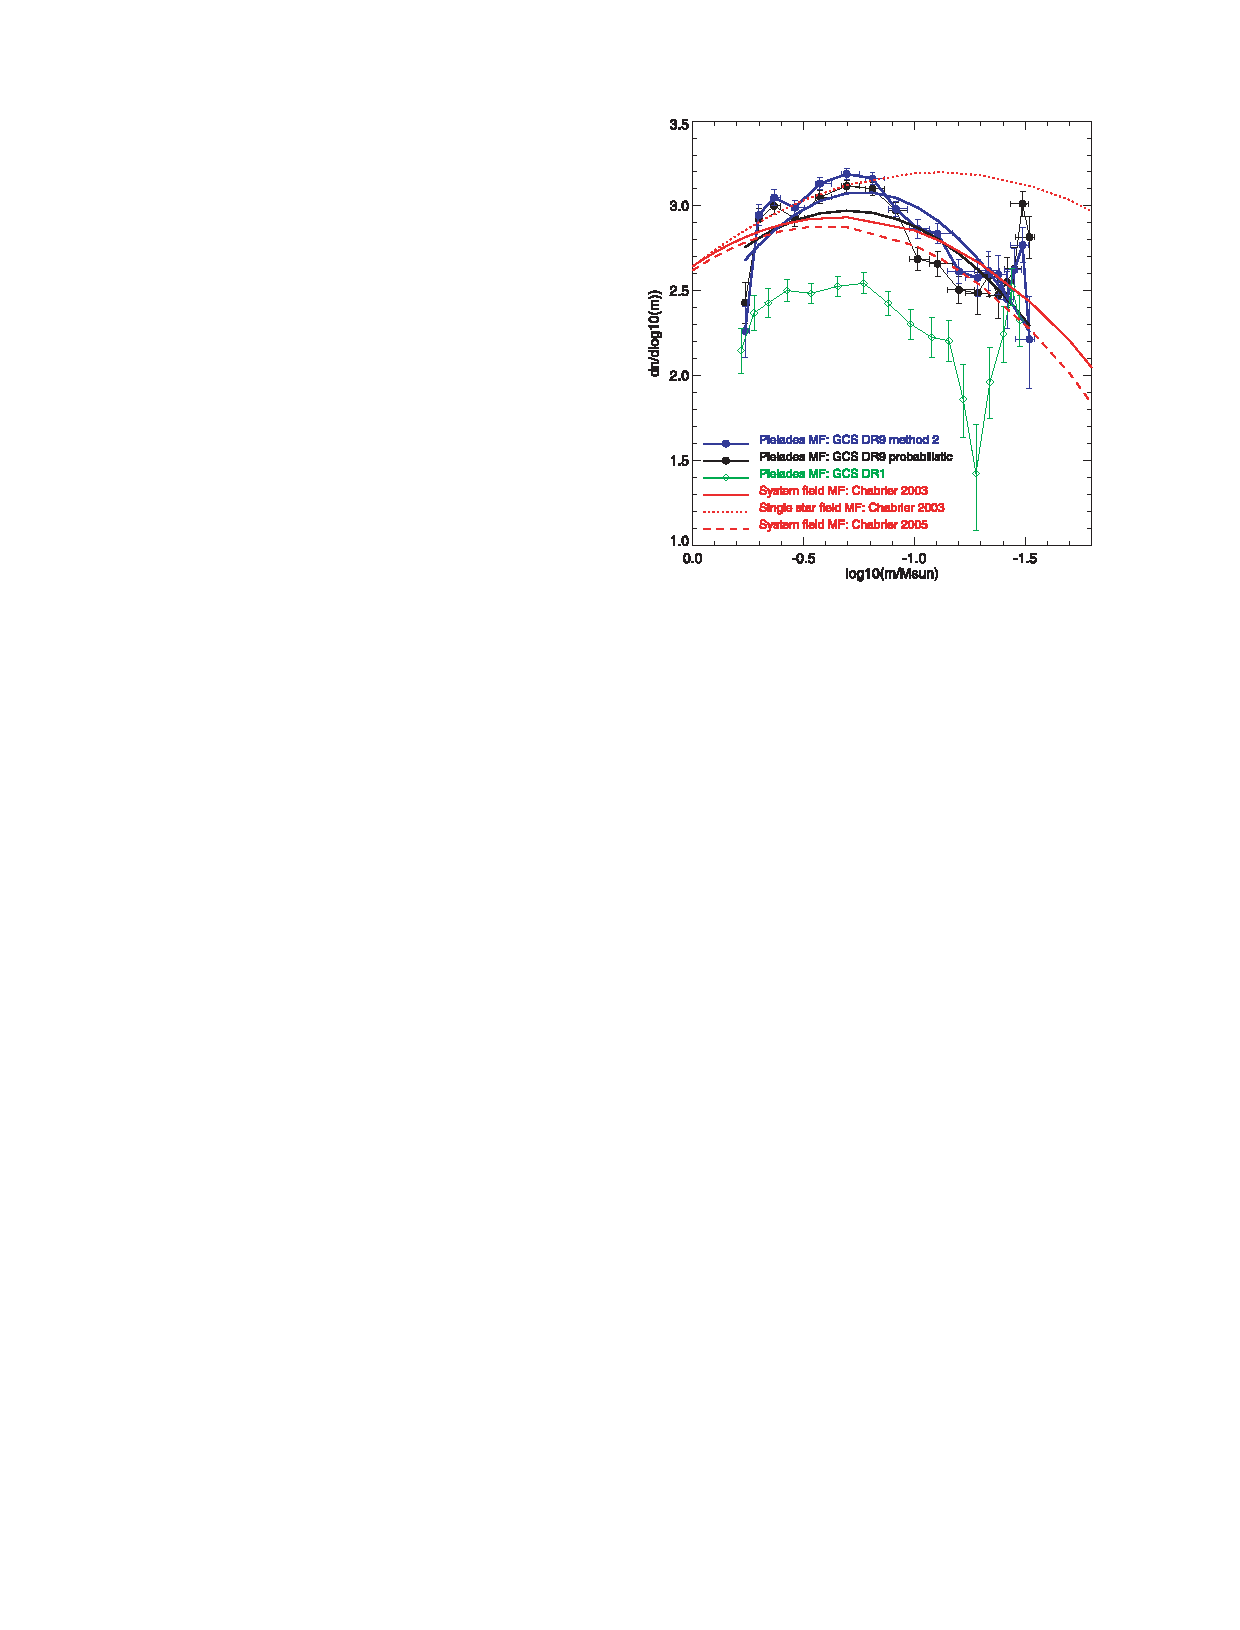
\includegraphics[height=8cm]{background/Figures/F9b_Lodieu2012.pdf}
\caption{Pleiades present day mass distribution from \citet{Lodieu2012}. GCS stands for Galactic Cluster Survey. The first and last two points must be treated with caution due to saturation and contamination at the bright and faint ends, respectively. Reproduced from Figure 9 of \citet{Lodieu2012}, \textit{\usebibentry{Lodieu2012}{Title}}, \usebibentry{Lodieu2012}{Journal}, Vol. \usebibentry{Lodieu2012}{Volume}.}
\label{fig:massLodieu}
\end{center}
\end{figure}

\begin{figure}[ht!]
\begin{center}
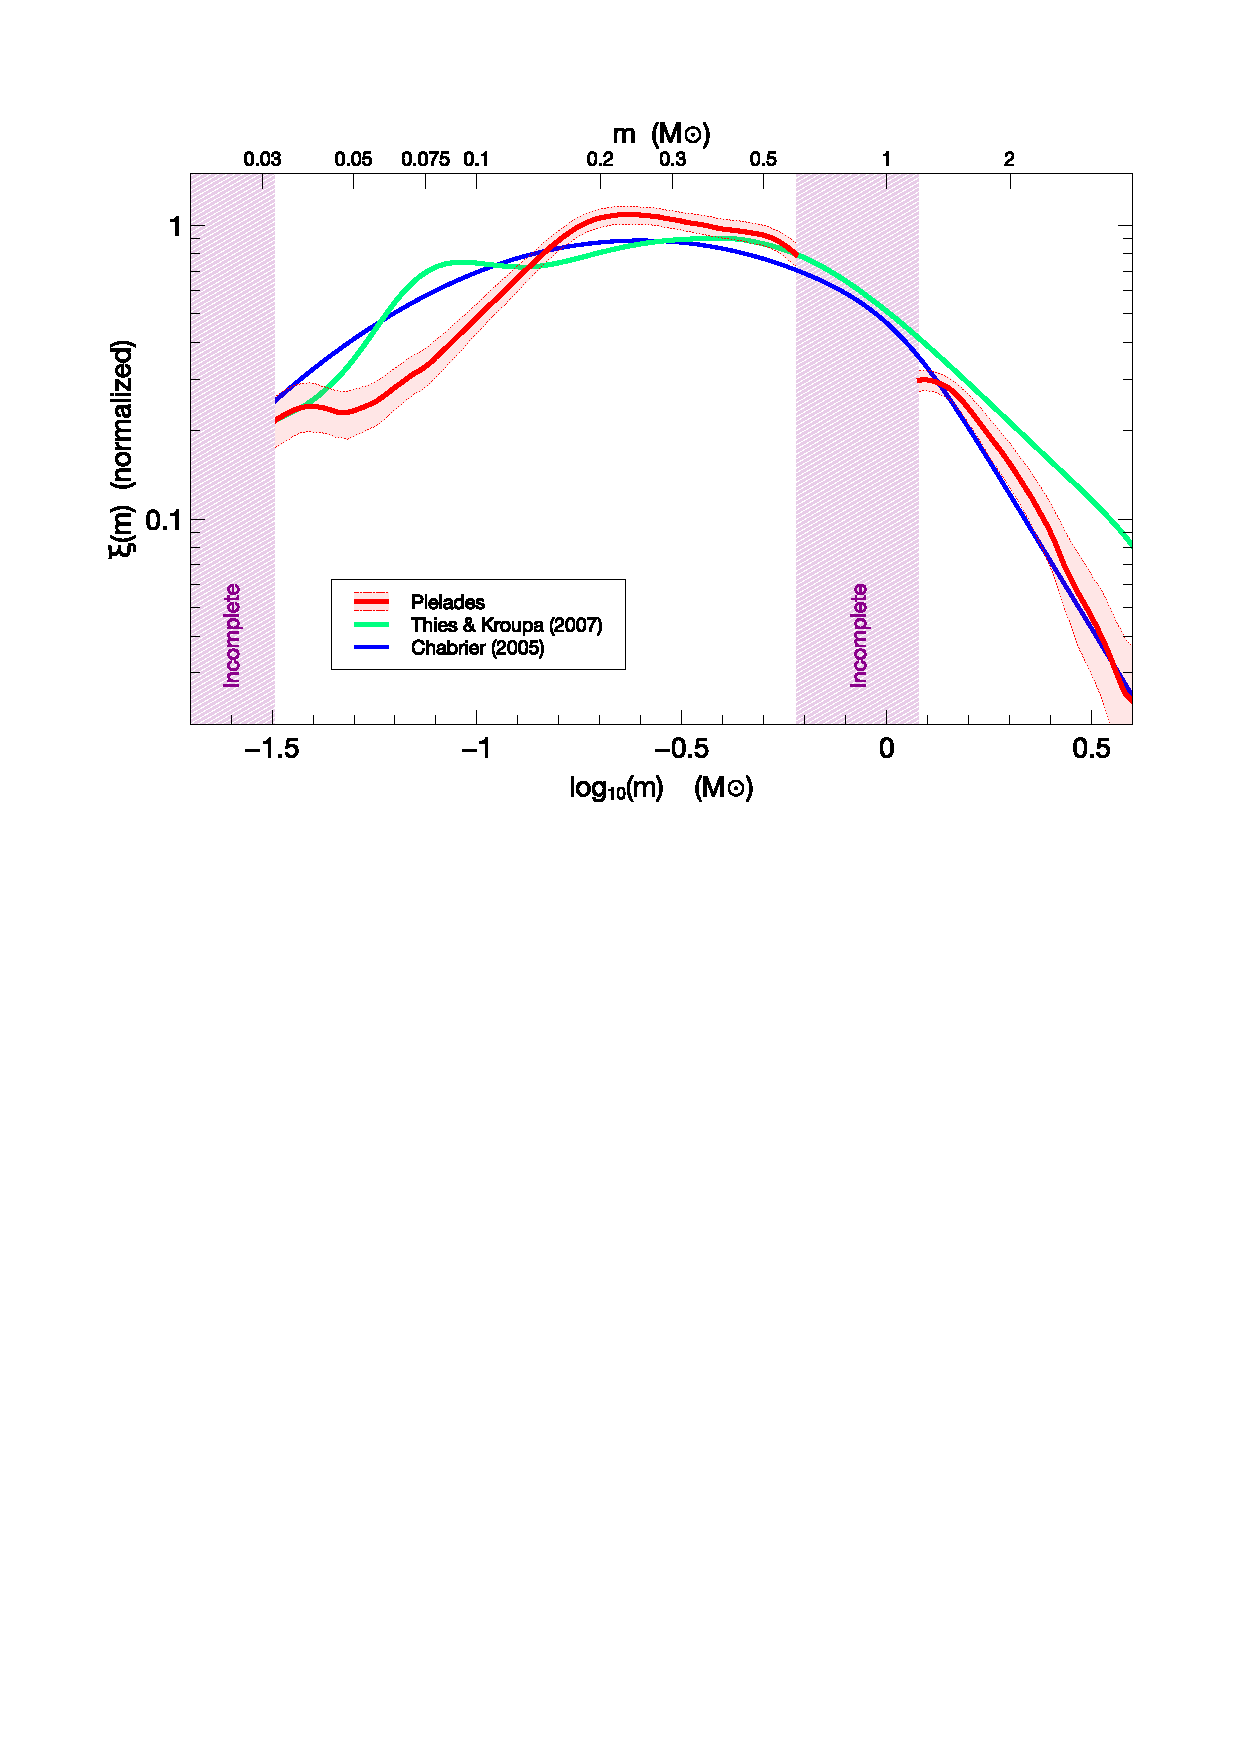
\includegraphics[height=8cm]{background/Figures/F9_Bouy2015.pdf}
\caption{Pleiades present day mass distribution  from \citet{Bouy2015} (red). \glspl{imf} from \citet{Chabrier2005}(blue) and \citet{Thies2007} (green) are also shown. Reproduced from Figure 9 of \citet{Bouy2015}, \textit{\usebibentry{Bouy2015}{Title}}, \usebibentry{Bouy2015}{Journal}, Vol. \usebibentry{Bouy2015}{Volume}.}
\label{fig:massBouy}
\end{center}
\end{figure}

\subsection{Total mass of the cluster}
Before ending this section I present a (non exhaustive) summary of the studies that provided an estimate of the total mass of the cluster.

The first record I found of the cluster total mass is that of \citet{1938AJ.....47...25T}. He estimated a total mass of $260 \,M_{\odot}$ assuming virial equilibrium. He also computed $200 \,\mathrm{M_{\odot}}$ using the Eddignton's mass-luminosity relation for objects brighter than $15$ mag in the visual band.

The subsequent works continue to report higher masses. \citet{1956MNRAS.116..296W} estimated a total mass of $337 \,\mathrm{M_{\odot}}$ using a polytrope model fitted to Hertzsprung's catalogue. He then mentions that taking into account Trumpler's data, the total mass should be about $500\,M_{\odot}$. 

\citet{Limber1962} computed the total mass in two ways. In the first one he assumed the cluster was virialised and obtained a mass of $900 \,M_{\odot}$. Using the luminosity function he estimated the lower limit to the total mass in $760 \,\mathrm{M_{\odot}}$. 

\citet{1970AJ.....75..563J} measured $470\,\mathrm{M_{\odot}}$ and $690\,\mathrm{M_{\odot}}$ using the luminosity distribution and the virial theorem, respectively. 

Later, \citet{1980IAUS...85..157V}  determined a total mass of $2000 \,\mathrm{M_{\odot}}$ using the virial theorem, a mean individual mass of $2\,\mathrm{M_{\odot}}$, and a velocity dispersion of $0.7\,\mathrm{km \cdot s^{-1}}$ in each spatial direction. 

\citet{1995JKAS...28...45L} measured $700 \,\mathrm{M_{\odot}}$ using the luminosity distribution and a mass-luminosity relation. 

\citet{Pinfield1998} fitting a King profile to the \gls{psd} of the cluster members obtained $735\,\mathrm{M_{\odot}}$. 

\citet{Adams2001} counting individual masses of candidate members within $5.5^{\circ}$ obtained a total mass of $690 \,\mathrm{M_{\odot}}$. 

\citet{Converse2008} found $820 \,\mathrm{M_{\odot}}$ after adding the individual masses of 1245  candidate members of \citet{Stauffer2007}. To obtain these masses they  transformed the $K$ and $I-K$ magnitude and colour into masses using the mass-luminosity relation given by the theoretical isochrone models of \citet{1998A&A...337..403B}. Later, \citet{Converse2010} redid their analysis and found the total mass to be $870\pm35\,\mathrm{M_{\odot}}$.

%\section{The current dynamical scenario}
%The most important sources of gravitational interactions affecting individual objects are due to: other individual objects (like for example close encounters or binary interactions), the ensemble of individual objects (the potential of the cluster itself or its momentum), other ensembles of objects (interactions with other clusters or molecular clouds) and, the galactic potential (perturbations due to the disk, resonances, arms).
%
%\subsection{Pleiades time-scales}
%Pinfield equation 13 and 14

\section{The Pleiades DANCe DR2}
\label{sect:DR2}

The \glsfirst{ddr2} contains astrometric (stellar positions and proper motions) and photometric ($ugrizYJHK_s$) measurements for 1,972,245 objects. As explained in Chapter 1, the \gls{dance} data set has an heterogenous origin, which can be observed in Fig. \ref{fig:originDANCeDR2} where the patchy pattern arise from the combination of several surveys. The interested reader can find more the details of this data set and its processing in \citet{Bouy2013,Bouy2015}. Here, I briefly summarise its properties. Table \ref{tab:DR2properties} contains the basic statistics for the observables, while Table \ref{tab:DR2uncertainties} does it for the uncertainties. As an example, Fig. \ref{fig:pmuncert} shows the proper motions uncertainties as a function of the $i$ magnitude.

\begin{figure}[ht!]
\begin{center}
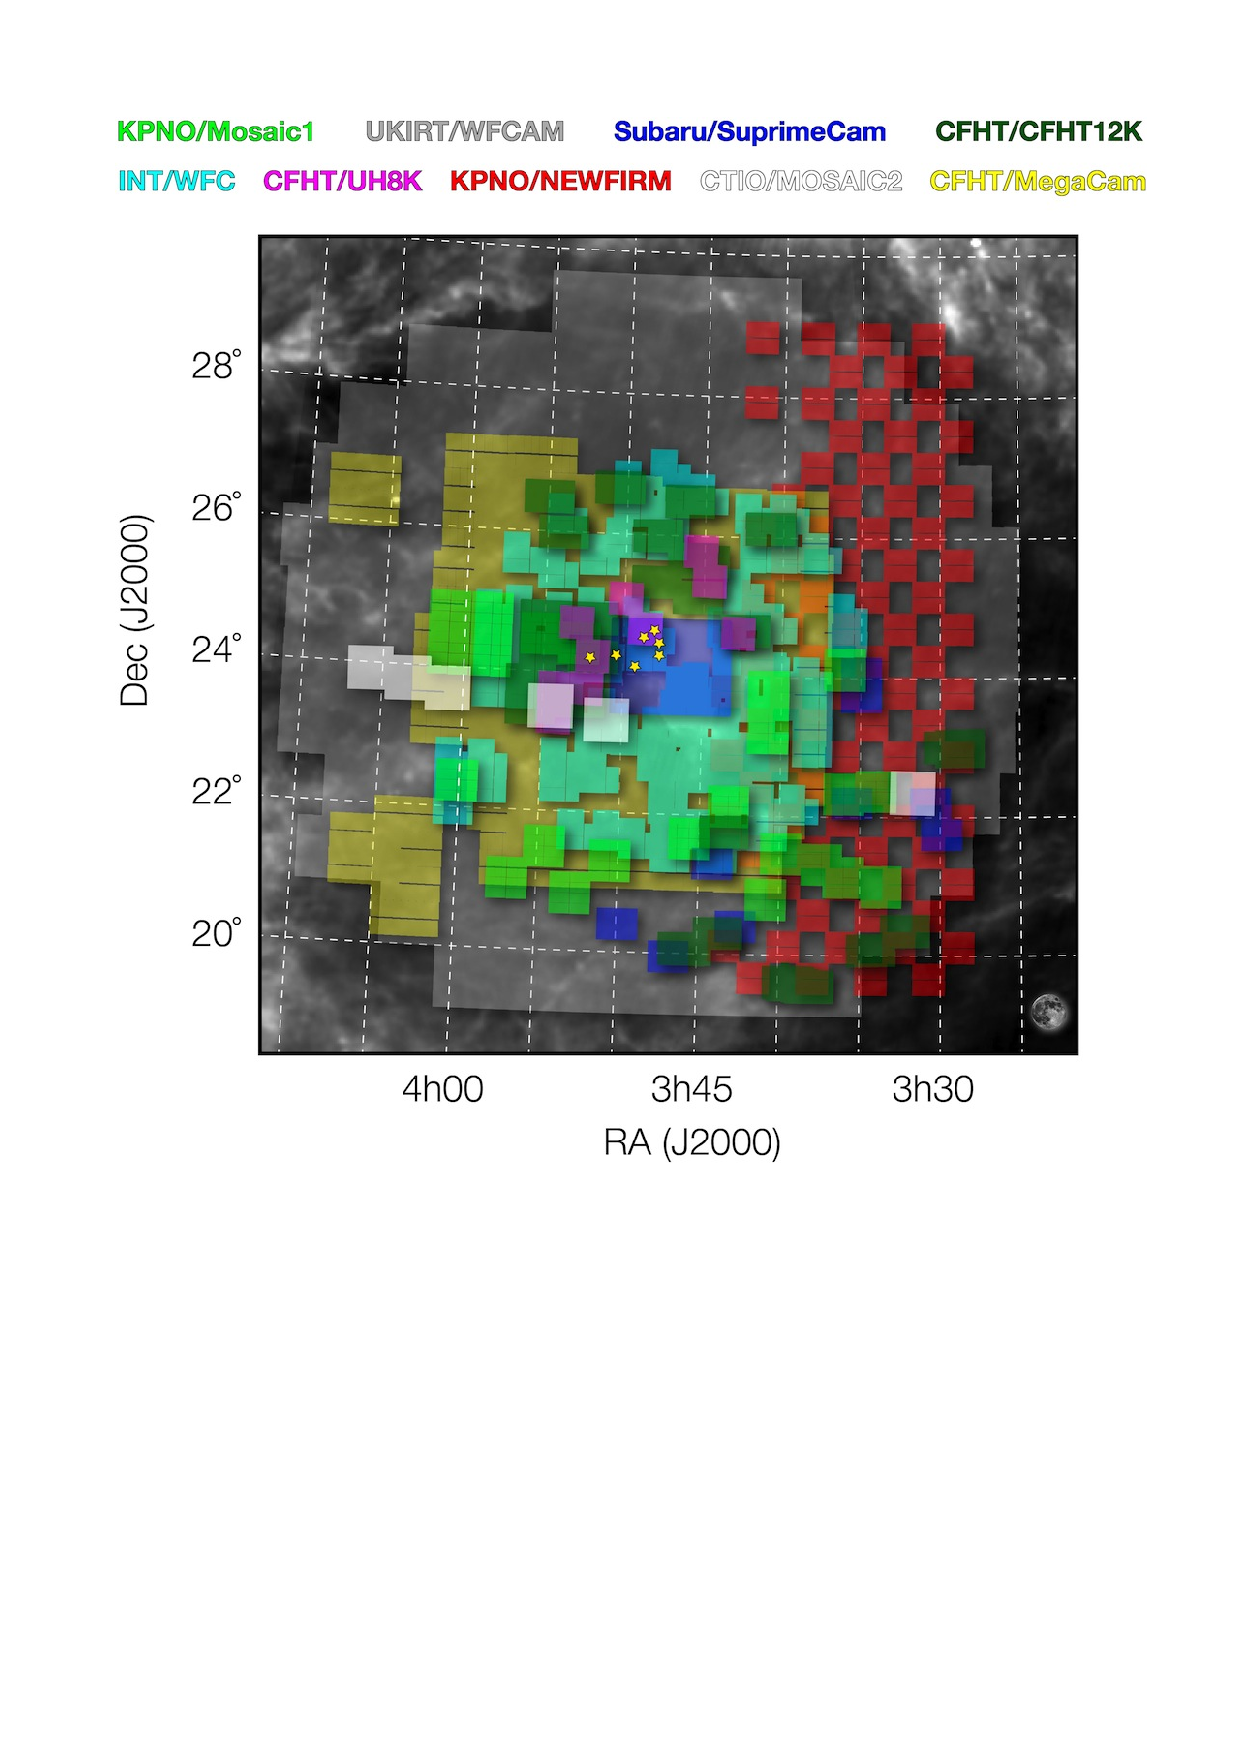
\includegraphics[width=\textwidth]{background/Figures/F1_Bouy2013.pdf}
\caption{Patchy composition of the \gls{ddr2}. The moon shows the scale, and the yellow stars correspond to the central brightest objects of the Pleiades cluster. As can be seen, the UKIDSS (UKIRT) survey provides the most homogeneous and extended coverage. Reproduced from Figure 1 of \citet{Bouy2013}, \textit{\usebibentry{Bouy2013}{Title}}, \usebibentry{Bouy2013}{Journal}, Vol. \usebibentry{Bouy2013}{Volume}.}
\label{fig:originDANCeDR2}
\end{center}
\end{figure}

\begin{table}[htdp]
\caption{Summary of the \gls{ddr2}.}
\begin{center}
\begin{tabular}{|c|c|c|c|c|c|c|c|}
\hline
Observable & Min. & 1st. Qu. & Median & Mean & 3rd. Qu. & Max. & NA's \\
\hline
\hline
RA [deg]&51.23 & 55.40 & 57.35 & 57.26 & 59.01 & 62.94 & 0\\
Dec. [deg] &19.12 &22.47 & 24.32 & 24.27  & 25.95 & 29.69 &0\\
$\mu_{\alpha} [mas\cdot yr^{-1}]$&-99.998& -6.060& -1.645& -1.240&3.401&99.996&0\\
$\mu_{\delta} [mas\cdot yr^{-1}]$&-99.997& -2.835&  2.548&  1.976&  7.017&99.989&0\\
u [mag]&13.6&20.4 &22.0 &21.6&23.3&25.2&1756374\\
g [mag]& 9.4   &19.6   &22.1   &21.1   &23.3   &25.5 &1492564\\
r [mag] &  8.4  &17.6   &21.3   &20.3   &22.6   &25.1   &1222853\\
i [mag] &  7.5  &20.0  &21.6  &21.0  &22.7  &25.5  &820861\\
z [mag]&11.2  &17.9  &19.3  &18.9  &20.2  &25.0  &697412\\
Y [mag]& 8.3  &17.2  &18.5  &18.1  &19.4  &24.2  &688144\\
J [mag]& 2.8  &16.7  &17.9  &17.5  &18.8  &23.1  &645469\\
H [mag]& 2.0  &16.1  &17.3  &16.9  &18.1  &20.9  &653682\\
$K_s$ [mag]& 1.8 &16.0&  17.0  &16.7  &17.7  &23.8  &561745\\
\hline
\end{tabular}
\end{center}
\label{tab:DR2properties}
\end{table}%

\begin{table}[ht!]
\caption{Uncertainties of the \gls{ddr2}.}
\begin{center}
\begin{tabular}{|c|c|c|c|c|c|c|c|}
\hline
Observable & Min. & 1st. Qu. & Median & 3rd. Qu. & Max. &Mean\\
\hline
\hline
RA [deg]&8.900e-08 &9.270e-07&1.933e-06&4.037e-06&2.156e-02&3.173e-06\\
Dec. [deg] &8.900e-08&9.270e-07&1.932e-06&4.037e-06&2.156e-02&3.173e-06\\
$\mu_{\alpha} [mas\cdot yr^{-1}]$&2.01e-01 &1.89e+00& 4.35e+00& 1.00e+01& 1.49e+22&3.99e+16\\ 
$\mu_{\delta} [mas\cdot yr^{-1}]$&1.92e-01 &1.89e+00 &4.35e+00 &1.00e+01 & 4.71e+09&1.42e+04\\
u [mag] &3.73e-04& 8.07e-03& 3.06e-02& 8.56e-02& 2.17e-01&5.48e-02\\
g [mag] &1.72e-01 & 1.02e-02&  3.90e-02 & 7.90e-02 & 1.82e+00&5.34e-02\\
r [mag] & 2.83e-04 & 1.54e-02& 4.88e-02 &1.04e-01& 1.42e+00&6.34e-02\\
i [mag] & 4.04e-04 & 9.03e-03&  2.73e-02& 5.85e-02& 2.40e+00&4.37e-02\\
z [mag] & 6.49e-04& 5.62e-02& 9.16e-02& 1.85e-01& 3.12e+00&1.34e-01\\
Y [mag] & 3.00e-02& 5.21e-02& 6.50e-02& 1.03e-01& 9.01e+00&8.56e-02\\
J [mag] & 1.60e-02& 5.24e-02& 6.66e-02& 1.04e-01& 8.89e+00&8.57e-02\\
H [mag] & 1.40e-02& 5.28e-02& 7.04e-02& 1.10e-01& 1.00e+01&8.85e-02\\
$K_s$[mag]&1.40e-02& 5.75e-02& 8.17e-02& 1.32e-01& 3.88e+01&1.04e-01\\
\hline
\end{tabular}
\end{center}
\label{tab:DR2uncertainties}
\end{table}%

\begin{figure}[ht!]
\begin{center}
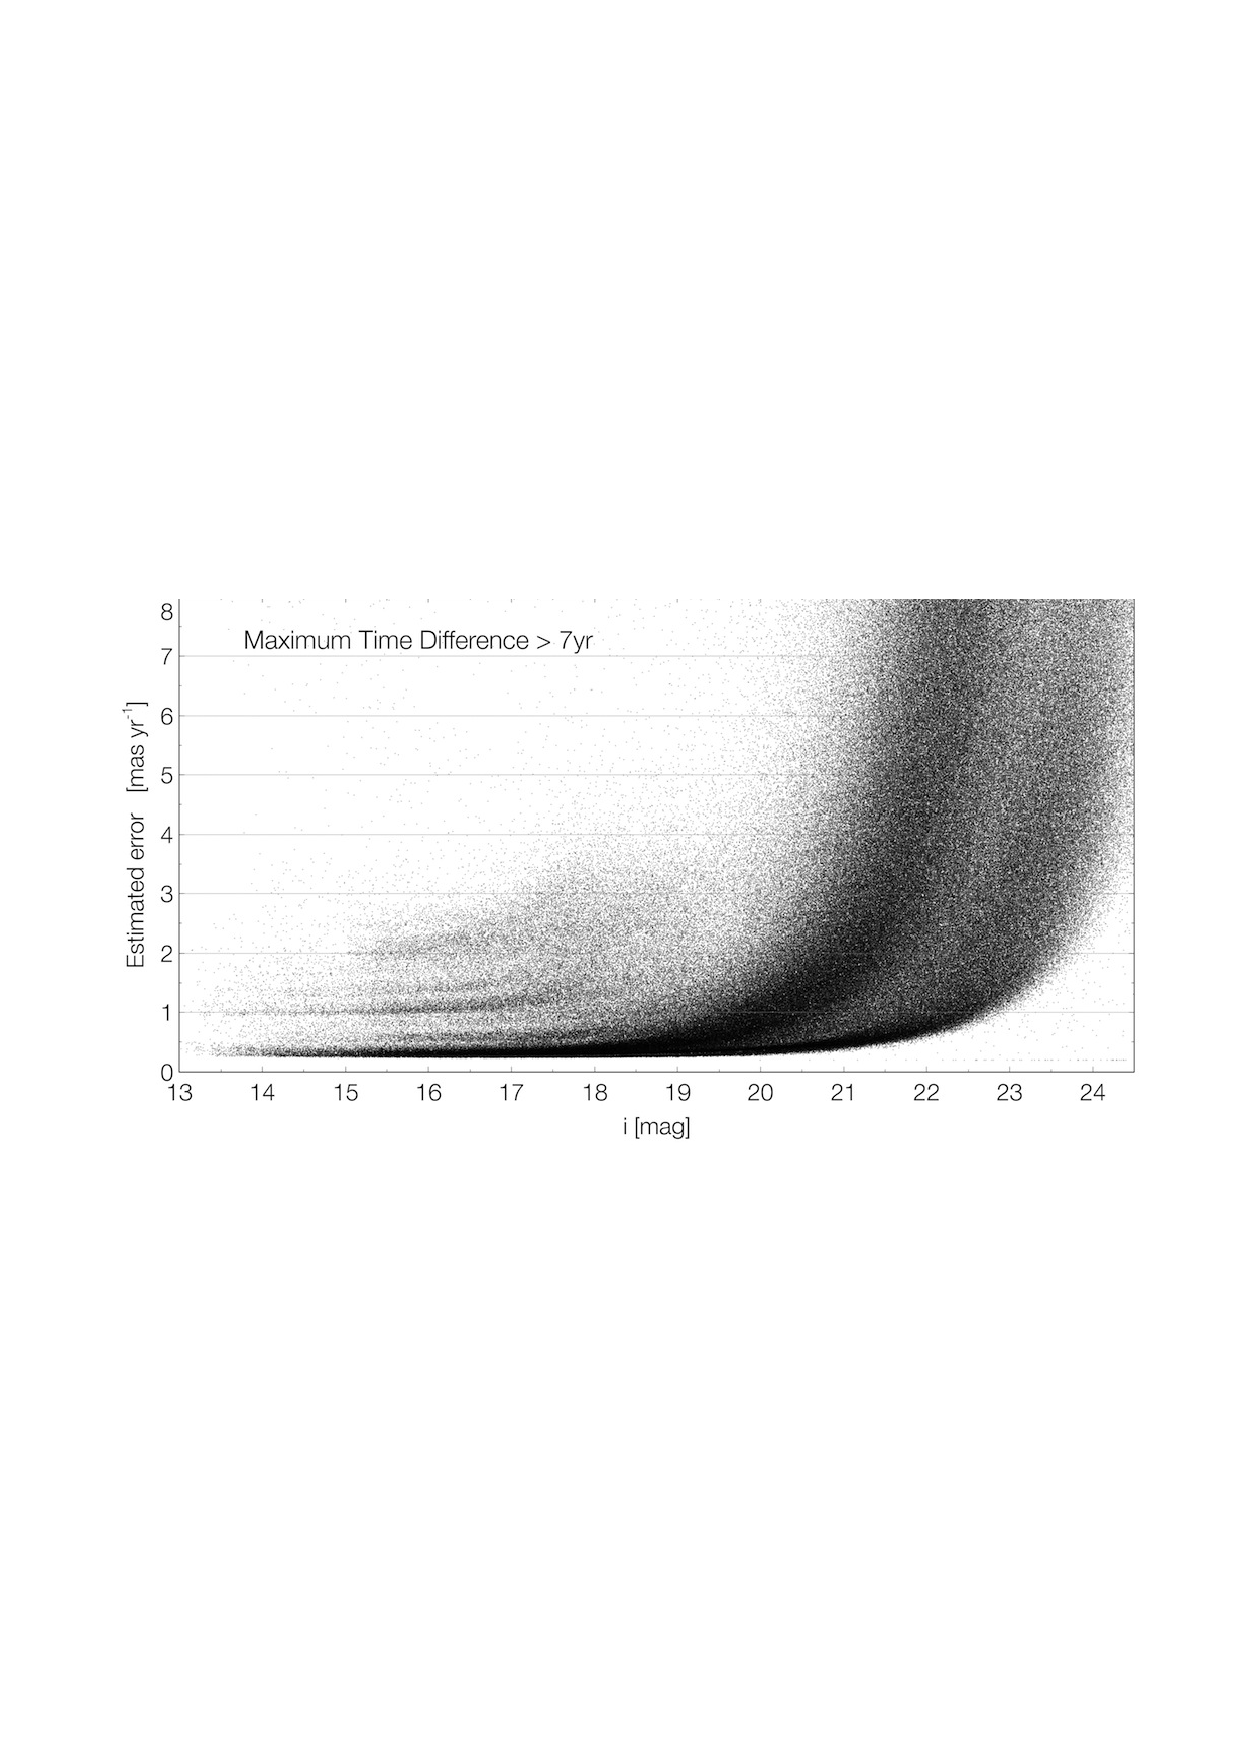
\includegraphics[height=8cm]{background/Figures/F12_Bouy2013.pdf}
\caption{Proper motion uncertainty as a function of the photometric magnitude in the $i$ band. Reproduced from Figure 12 of \citet{Bouy2013}, \textit{\usebibentry{Bouy2013}{Title}}, \usebibentry{Bouy2013}{Journal}, Vol. \usebibentry{Bouy2013}{Volume}.}
\label{fig:pmuncert}
\end{center}
\end{figure}

\subsection{Selection of observables}
\label{sect:RF-2}
\sloppy
The \gls{ddr2} contains the positions R.A., Dec. (in the following $\alpha$ and $\delta$), proper motions, $\mu_{\rm{R.A.}},\mu_{\rm{Dec.}}$, and photometric $ugrizYJHK_s$ bands, of almost two million sources on the vicinity of the Pleiades clusters. Although these 13 observables carry information valuable to discriminate cluster members from field objects, not all of them do it in the same way. \citet{Sarro2014} give a detailed analysis of the capacity of the previous observables (with the exception of the stellar positions) to discriminate between cluster members and field population. These authors use random forest to select the observables that were the most discriminant. They find that the proper motions ($\mu_{R.A.},\mu_{Dec.}$) and the photometric bands $rizYJHK_s$ are the most discriminants. 

Since most the objects with a missing $r$ band occur at the faint end of the cluster sequence, \citet{Sarro2014} train their model (see Section \ref{sect:current_methodologies}) in two stages. In the first stage, they use all literature candidate members with observed $r$ band. In the second stage, they discard the $r$ band observations and continue training their model with objects in which the $r$ band was missing. In a subsequent analysis using roughly the same methodology, \citet{Bouy2015} skipped the first training stage and worked only with the RF-2, which also excludes the $z$ band.

Therefore, in the present work I use as a reference set the the proper motions, $\mu_{\alpha},\mu_{\delta}$, the photometric bands $Y,J,H,K_s$, and the colour index $i-K_s$, with the addition of the stellar positions  $\alpha$ and $\delta$. This decision roots in the following reasons.

\begin{itemize}

\item First, \citet{Sarro2014} prove that these observables (excluding the stellar positions) are amongst the most discriminant ones in the \gls{ddr2}. 

\item Second, this set corresponds to the one used by \cite{Bouy2015}, thus, it will enable us to perform a direct comparison and validation with their results. 
However, observables used by \cite{Bouy2015} and the ones use in the present work are not exactly alike. While here I use the $Y$ band alone, \citet{Bouy2015} use the colour index $Y-J$. Originally, I tested the methodology with this $Y-J$ colour index but the contamination resulting from it was higher than that resulting from the use of the $Y$ band. This is a consequence of how the intrinsic dispersion of the cluster photometric sequence is modelled. The details of it will be shown in Section \ref{subsect:cluster}. Here suffices to say that the photometric model describes the cluster sequence dispersion with a constant width across the $i-K_s$ colour index. The dispersion of the cluster sequence in the $Y-J$ vs. $i-K_s$ colour-colour diagram varies greatly across $i-K_s$ contrary to the elatively stable dispersion in the $Y$ vs $i-K_s$ \gls{cmd}. This effect can be observed in Figure \ref{fig:Y-JvsY}, where the candidate members of \citet{Bouy2015} (blue dots) are depicted, together with the \gls{ddr2} density (black contour lines), in the colour-colour diagram $Y-J$ vs. $i-K_s$, and the  \gls{cmd} $Y$ vs $i-K_s$.  Therefore, the use of $Y-J$ results in larger contamination in those regions where the true clusters sequence is narrower than the average model. Future steps will be take to include more colour indices in the reference set of observables.

\end{itemize}

\begin{figure}[htp!]
\begin{center}
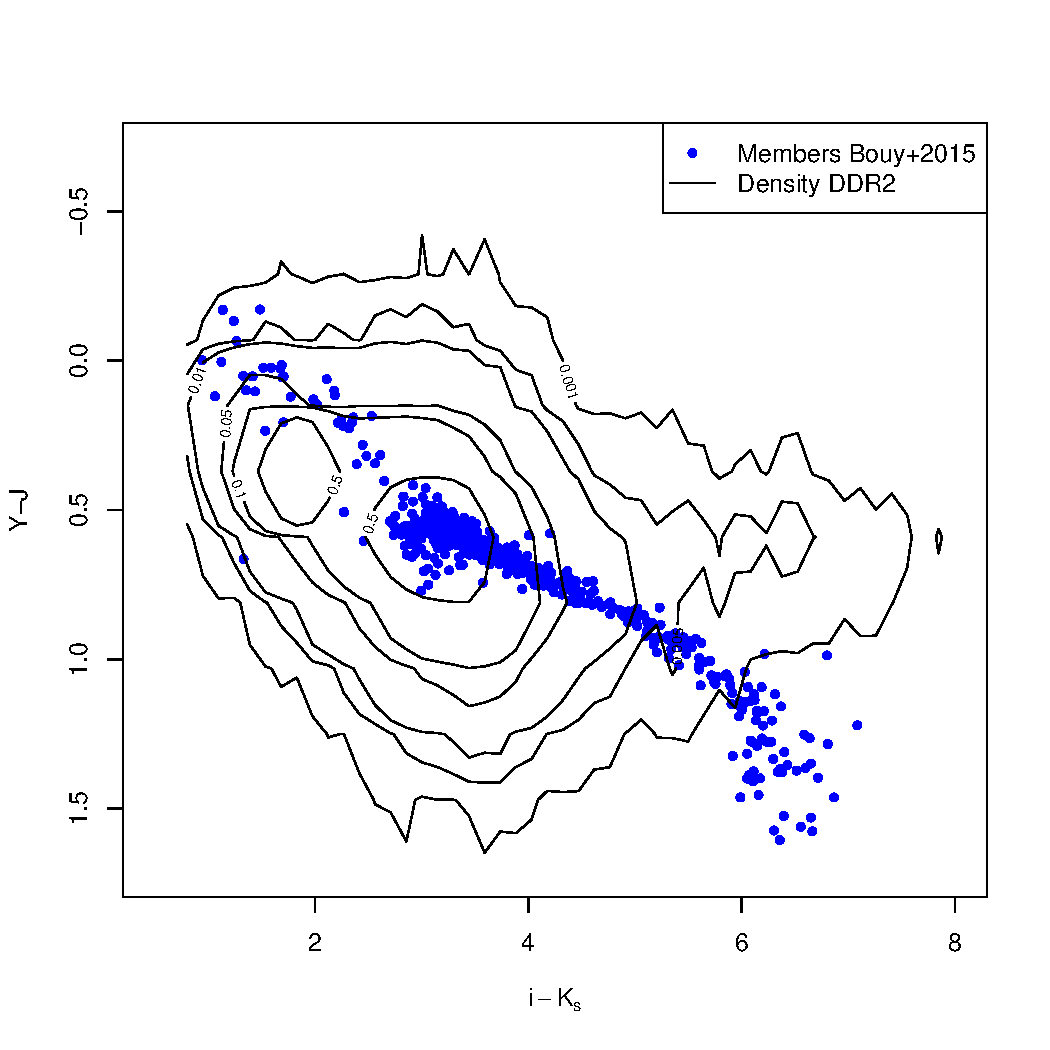
\includegraphics[page=1,width=0.47\textwidth]{background/Figures/Y-J.pdf}
\includegraphics[page=2,width=0.47\textwidth]{background/Figures/Y-J.pdf}
\caption{Candidate members of \citet{Bouy2015}, blue dots, together with the density of the \gls{rdr2} data set, black contours, in the colour-colour  diagram $Y-J$ vs. $i-K_s$ (left) and \gls{cmd} $Y$ vs $i-K_s$ (right).}
\label{fig:Y-JvsY}
\end{center}
\end{figure}
 

Concerning the stellar positions $\alpha$ and $\delta$, neither \citet{Bouy2015} nor \citet{Sarro2014} use them in their analyses. Thus, I will independently analyse the: i) the kinematic and photometric distributions of the cluster population, and ii) the \gls{psd}. This decision roots in the following reasons.

\begin{itemize}

\item To fulfil the objective of the \gls{dance} project (see Section \ref{sect:DANCeproject}), the inventory of kinematic and photometric distributions of the \glspl{nyc} must be obtained with an homogenous methodology. The \gls{dance} \gls{nyc} targets (see Tables \ref{tab:maintargets} and \ref{tab:secondarytargets}) do not share similar projected spatial density profiles; while Taurus, Ophiucus and the Trapezium are extended \cite[see for example][]{simon1997}, the Pleiades is almost radially symmetric \citep{Raboud1998}. Thus, including the spatial information together with the proper motions and photometry would require completely different models for the \gls{psd} of different clusters. That would result in non-homogenous methodologies that would bias any comparison between the derived \gls{pdsmd} of these clusters.
\item To validate the results of the present work, which will be conducted in the Pleiades cluster, we must compare them with similar results under the most similar conditions. Since \citet{Bouy2015,Sarro2014} do not include the stellar positions in their observables, I do that as well. 
\item Almost all previous analyses of the Pleiades \gls{psd} use King profile (see Section \ref{sect:PSD}) without providing any further reason beyond its physical interpretability, which nevertheless remains a good one. Thus, we decided to perform a Bayesian model selection analysis to compare how well the common surface density profiles, included the King's one, reproduce the Pleiades \gls{psd}. The results of this analysis have been submitted to the $A\&A$ journal.
\end{itemize}

As will be described in Section \ref{subsect:cluster}, the cluster photometric sequence, in each magnitude, is modelled by functions in which the parameter is the \emph{true} \gls{ci} (details for this decision will be given in Section \ref{sect:cluster_ph}. Thus, our photometric set of observables is made of the colour index $\gls{ci}=i-K_s$ and the photometric bands $Y,J,H$ and $K_s$. 

\subsection{Data preprocessing}

Since both photometry and proper motions carry crucial information for the disentanglement of the cluster population, we restrict the data set to only those objects with observed proper motions, and also at least two photometric entries in our photometric set ($i-K_s,Y,J,H,K_s$). Objects with only one photometric entry, although theoretically could be included in the data set, are left aside due to computational reasons. Their treatment requires selection statements to choose between the univariate and multivariate computational libraries that proved to be computationally expensive.

The previous restrictions exclude 22 candidate members of \citet{Bouy2015}, which have only one observed value in the photometry. For these particular objects, we compute their marginal proper motion membership probability a posteriori, once the parameters of the model were inferred. The mode and 16 and 84 percentiles of their membership probabilities are listed in Table \ref{tab:22excluded}. Only four of these 22 objects have membership probabilities below 0.5, which may indicate they are contaminants. Since these membership probabilities were computed using only the kinematic information, these four members could not be discarded as probable candidate members.

In the following, whenever I mention the Pleiades candidate members of \citet{Bouy2015}, I refer to the 1988 objects in the \gls{ddr2} with \citet{Bouy2015} membership probabilities grater than 0.75, and with at least two observed values in the photometry.

\begin{table}[htdp]
\caption{Membership probabilities of the 22 excluded candidate members of \citet{Bouy2015}.}
\begin{center}
\begin{tabular}{|c|c|c|c|}
\hline
ID DANCe & $P_{16}$ & Mode & $P_{84}$\\
\hline
\hline
J035106.55+211604.3 &0.751182& 0.7774335&    0.785560\\
J035057.42+240630.8 &0.792295& 0.8090186&   0.829541 \\
J034704.76+252249.8& 0.701193& 0.7319624 &   0.750745\\
J034725.80+250832.7 &0.789872& 0.8169538 &  0.827954 \\
J034437.44+250815.6 &0.762013& 0.7773114 &   0.798125\\
J035125.88+244738.6& 0.883488& 0.9007972 &  0.905823 \\
J034235.64+215029.7 &0.838538& 0.8662402 &  0.871439 \\
J034516.66+243432.1 &0.862284& 0.8666611 &   0.881004\\
J034926.12+235714.8& 0.852537& 0.8606685 &  0.866286 \\
J034920.60+244635.9 &0.923319& 0.9270399 &  0.935532 \\
J035300.63+233252.3 &0.762996& 0.7747163 &  0.781901 \\
J034606.52+235020.2& 0.928688& 0.9333306 &  0.940772 \\
J035040.89+245657.7 &0.509435& 0.5215143 &  0.530379 \\
J034845.33+233124.8 &0.260551& 0.2650812 &  0.275513 \\
J034713.67+234953.3& 0.814689& 0.8489593 &  0.855902 \\
J034546.48+234743.0 &0.897035& 0.9098442 &  0.912059 \\
J034548.95+235110.2 &0.933892& 0.9376429 &   0.945558\\
J035202.26+242148.1& 0.248011& 0.2649874 &   0.305949\\
J035313.22+235540.8 &0.518388& 0.5425345 &  0.553376 \\
J034425.60+244052.5 &0.581242& 0.5902633 &  0.602096 \\
J035518.38+245637.2& 0.198074& 0.2087989 &  0.252831 \\
J035418.93+252944.0& 0.366009& 0.3760922 &  0.386213 \\
\hline
\end{tabular}
\end{center}
\label{tab:22excluded}
\end{table}%


Furthermore, we restrict the lower limit of the \gls{ci} to the value of the brightest cluster member, \gls{ci}=0.8 in the \gls{ddr2} data set (The actual value is \gls{ci}=0.93, see Table \ref{tab:rddr2_cluster}, but 0.8 was chosen conservatively to include the uncertainty). We do not expect to find new bluer members in the bright part of the \glspl{cmd}. In the Tycho+\gls{dance} data set \citep{Bouy2015}, which also comprises the bright side of the cluster sequence, the bluer candidate member of \citet{Bouy2015} has a \gls{ci}=0.67. This shows that the cut at 0.8 is reasonable for the fainter \gls{ddr2} data set. 

Also, we set the upper limit of the \gls{ci} to \gls{ci}=8, which is one magnitude redder than the colour index of the reddest known cluster member. This value allows for possible new discoveries. Due to the sensitivity limits of the \gls{ddr2} survey in $i$ and $K_s$ bands,\cite[$i\sim23$ mag and $K_s\sim18$ mag, see Appendix A of][]{Bouy2015}, the 262 objects with a \gls{ci} grater than this limit have $K_s$ magnitudes brighter than 16 mag. This combination of \gls{ci} and $K_s$ magnitude is clearly incompatible with the cluster sequence of \citet{Bouy2015} (see Fig. \ref{fig:incompatible_objects}), which allows us to remove  them from the data set.

Although formally these two cuts in the observed $\gls{ci}$ (and only in objects with observed \gls{ci}) are not needed for the statistical analysis (which accounts for this truncation, see Section \ref{subsect:cluster}), they nevertheless improved significantly the computing time required for it. If we were to include these objects, the resulting \gls{ci} range (\gls{ci}$\in[-6,12.5]$) would have been 2.5 times larger than the \gls{ci}$\in[0.8,8]$. Thus, increasing in the same amount the computing time of the analysis (for more details, see Footnote \ref{foot:extendedCI} on page \pageref{foot:extendedCI}).

\begin{figure}[ht!]
\begin{center}
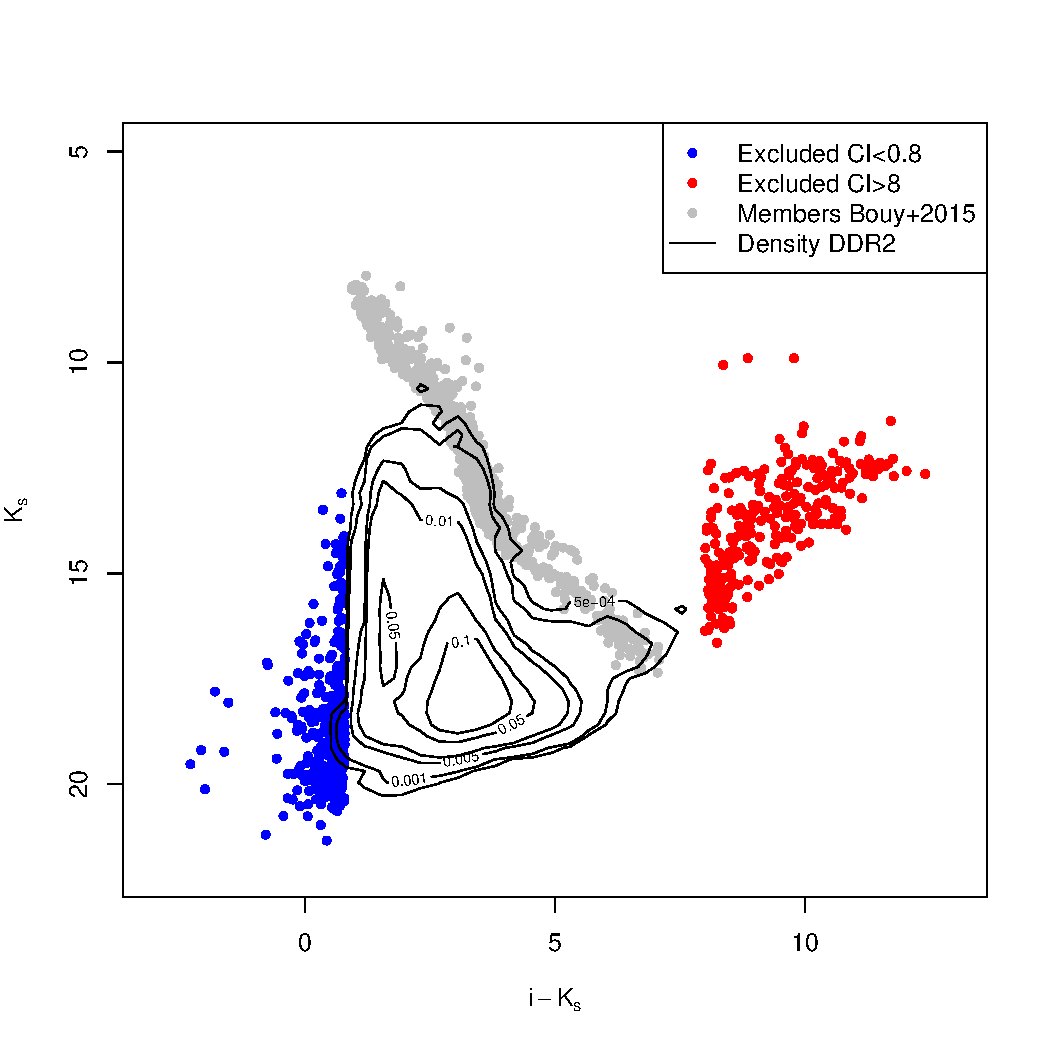
\includegraphics[width=\textwidth]{background/Figures/ColourCuts.pdf}
\caption{$K_s$ vs \gls{ci} \gls{cmd} showing the density (black contour lines) of all objects (with observed entries in this \gls{cmd}) in the \gls{ddr2}. Also shown, the candidate members of \citet{Bouy2015} (grey dots), and the objects excluded by the cuts at \gls{ci}=0.8 (blue dots) and \gls{ci}=8 (red dots). See text for details.}
\label{fig:incompatible_objects}
\end{center}
\end{figure}

With the previous restrictions, the number of sources in the \gls{ddr2} reduces to 1 424 893 objects, where the large number of rejected objects ($\sim 500\, 000$) results from a completely missing photometry.

There is no selection of objects based on proper motions or sky positions besides those intrinsic to the catalogue. The latter are: i) the proper motions are truncated to $\mu_{\alpha} \leq 100$ mas yr$^-1$ and $\mu_{\alpha} \leq 100$ mas yr$^-1$, and ii) the sky positions have a patchy composition (see Fig. \ref{fig:originDANCeDR2}), which reaches its end with the spatial coverage of \gls{ukidss}.

In the following sections I present two faces of an important element in any observational analysis: the non-observed data. One face corresponds to data from which no record exists. The second face corresponds to data in which some information is lost (i.e. the data is partially observed). For the first case I will estimate the region, in the observable space, where the data at hand (which comprises also the partially observed data) can be assumed as  representative of the true population. For the second case, I will estimate the probability distributions of the partially observed data in each of the observables. These two elements will be useful for the statistical analysis presented in Chapter \ref{chap:BHM}, and the results shown in Chapter \ref{chap:Results}.      

\subsection{Completeness}
\label{sect:ddr2_completeness}

In the astronomical community, the completeness of a sample is defined as the percentage of the sources in the true population that are present in the sample. It is common to refer to a sample as complete if its completeness is 100\%, otherwise, its completeness percentage or fraction is indicated. Thus, for example, a sample is said to be complete in volume, if it contains all the sources within a certain volume.Also, a sample is said to be complete until certain magnitude if it contains all objects up to certain limiting magnitude. The question then turns in knowing how many sources from the true population are within the limits we are interested in. This question has not a simple answer, and often a complex model have to be assumed. 

Since one of the objectives of this work is to obtain the statistical distributions of the cluster population, it is important to establish these limits for all the observables.

The photometric completeness of the \gls{ddr2} is difficult to estimate due to its heterogeneous origin (e.g. see Figure \ref{fig:originDANCeDR2}). The variety of instruments, sensitivity in each of them, and integration times, makes this task overwhelming. Nevertheless, \citet{Bouy2015}, in their Appendix A, give rough estimates of these limits for the $i$ and $K_s$ bands. To estimate these limits in all the bands, I make the simplistic assumption that the number of sources in the region of the sky occupied by the \gls{ddr2} grows as a power-law\footnote{The brigthness of an object vanishes proportionally the square of its distance. Thus, under the assumption that sources are uniformly distributed in space, the number of observed sources is expected to grow quadratically with brightness.} in the observed photometric magnitude. This assumption is of course very simplistic since the Pleiades cluster and the galaxy itself introduce inhomogeneities that prevent this model. In spite of that, as can be seen in Figure \ref{fig:completeness}, which shows the distribution of sources in the \gls{ddr2} (resulting from the restrictions of the previous section) as a function of the photometric magnitudes, this assumption is correct in most of the photometric domain. However, at certain points, the power-law behaviour stops and the number of sources rapidly falls. In the following, I will assume that the survey is whenever its distribution of sources follows that of the power-law.

In addition, \citet{Bouy2015} mention that, due to the heterogeneous origins of the \gls{ddr2} data set, the spatial coverage is also not homogeneous. To remedy this issue, they identify a region with complete spatial coverage. They assume it to be the inner three degrees of the cluster (see Fig. \ref{fig:originDANCeDR2}). Then, they restricted their photometric analysis to this spatially complete region. Doing so, results in a sample of candidate members that is spatially biased. If any dynamical process has been set on the cluster such that the mass distribution of its members is not uniformly distributed in the space, then a spatial cut in a sample of candidate members will result in a bias on the mass distribution. One of such dynamical process is the mass segregation, which, as suggested by several authors \cite[][including the present work]{Adams2001,Converse2008,Converse2010} occurs in the Pleiades.

Thus, to avoid such spatial restriction, in the following I assume that the \gls{ukidss} survey \citep{2007MNRAS.379.1599L}, which is the most photometrically sensitive and spatially extended from among those that contribute to the \gls{ddr2} data set, provides homogeneous spatial and sensitivity coverage at faint magnitudes (see Fig. \ref{fig:originDANCeDR2}, and \citealt{Bouy2013}). According to \citet{2007MNRAS.379.1599L}, the completeness limits of the \gls{ukidss} survey are: $Y\sim20.16$, $J\sim19.56$,$H\sim18.81$, and $K\sim18.19$ magnitudes. In the $i$ band, which is not present in \gls{ukidss}, \citet{Bouy2015} estimate that the completeness limit is $i\sim23$ mag. Figure \ref{fig:completeness} shows the previous limits as vertical dotted lines.
As can be seen, these limits are optimistic for the \gls{ddr2}. Thus, after re-estimating them, I find the following values: $i\sim21.13$, $Y\sim19.25$, $J\sim18.6$, $H\sim18$, and $K\sim17.4$ magnitudes, which are also shown in Figure \ref{fig:completeness} as the vertical dashed lines. 

It is important to notice that, although avoiding the truncation to the central three degrees prevents the biases introduced in the sample of \citet{Bouy2015}, the \gls{ddr2} is nevertheless still biased by the truncation resulting from the spatial coverage of \gls{ukidss}.

The \gls{ddr2} is also incomplete in the bright end. The bright stars can saturate the detectors (i.e collect more photons than those allowed by the analogical to digital converters), and thus prevent to collect a complete sample of the bright sources. As stated in the Appendix A of \citet{Bouy2015} the \gls{ddr2} $JHK$ photometry is perfectly covered by the dynamics range of \gls{2mass} and \gls{ukidss}. Thus, I will assume that the \gls{ddr2} is complete in the bright end of these bands. On the other hand, the $Y$ and $i$ bands show effects of saturation. This is perfectly seen in Figure \ref{fig:completeness}, where the $Y$ distribution falls abruptly below $Y\sim13$. However, the case of the $i$ band is more intricate. This band comes from two main surveys: \gls{apass} in the bright end (with completeness limit $i\sim$15.5 mag., see bump in Figure \ref{fig:completeness}), and CFHT/MegaCam (yellow pattern in Figure \ref{fig:originDANCeDR2}) at the mid and low ends (with completeness limit at $i\sim21.2$). However, while \gls{apass} covers 100\% of the \gls{ddr2} sky area and its detectors do not saturates at the bright end (at least within the range covered by the \gls{ddr2} values), the detectors of CFHT/MegaCam, which covers just the central $3^\circ$ area, saturate at $i\sim13$, as indicated by \citet{Bouy2015}. This intricate pattern prevents an homogeneous completeness coverage. Thus, I make the conservative assumption that the $i$ band in the \gls{ddr2} is complete within the limits of $i\in [13,21.2]$ mag given by CFHT/MegaCam. 

\begin{figure}[ht!]
\begin{center}
\resizebox{\hsize}{!}{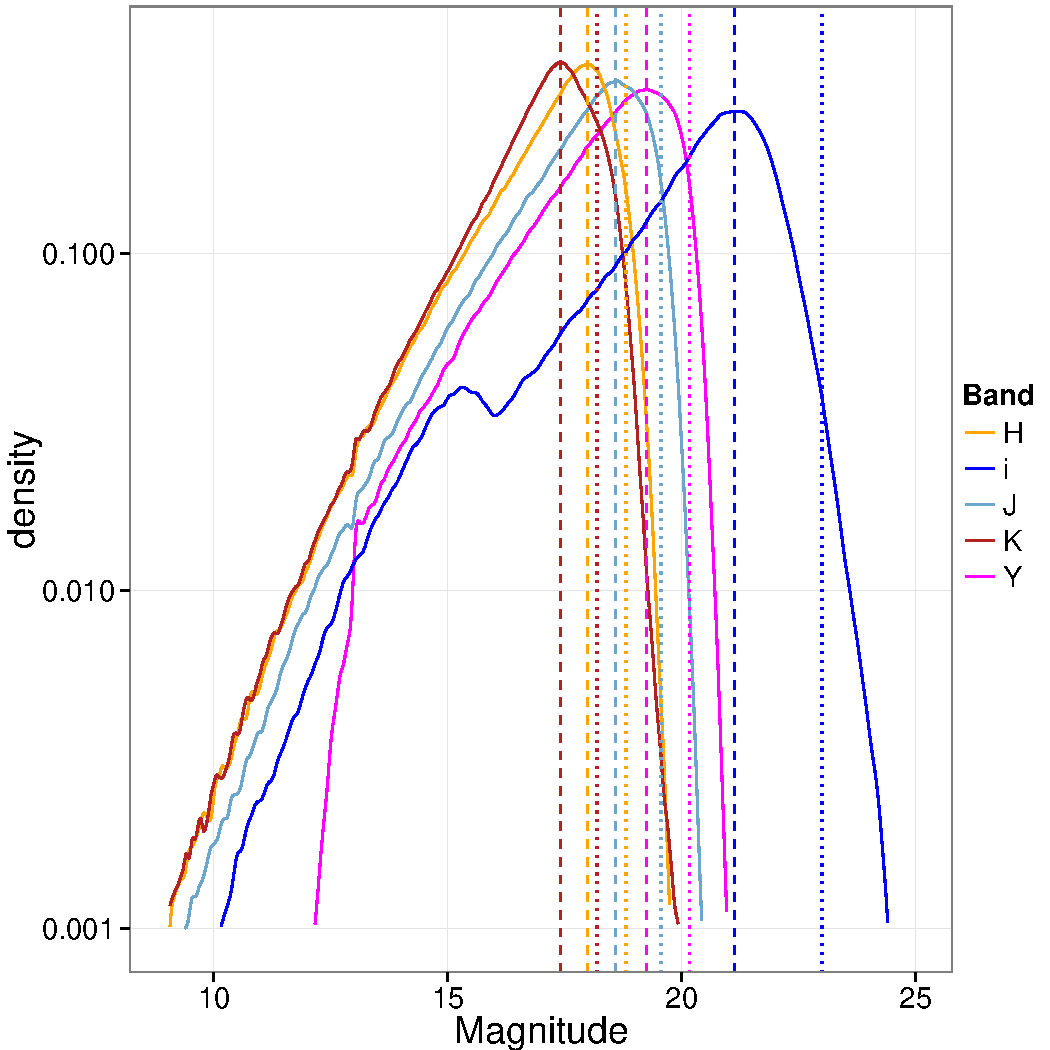
\includegraphics[width=0.5\textwidth]{background/Figures/MagnitudeDistributionsDDR2.pdf}}
\caption{Density of all \gls{ddr2} sources as a function of the observed magnitudes. The vertical dotted and dashed lines correspond to the completeness limits of the literature, and to those derived as the mode of the densities, respectively. The bump in the $i$ distribution at 15.5 mag corresponds to the completeness limits of the \gls{apass} survey.  See text and \citet{Bouy2015} for more details.}
\label{fig:completeness}.
\end{center}
\end{figure}

%As I will show in Chapter \ref{chap:BHM}, we are interested in the completeness limits of the $i - K_s$ colour index, which are defined by those of $i$ and $K_s$ together. In Fig. \ref{fig:completenessK+i}, I show the $K_s$ and $i$ 2d kernel density estimate of the \gls{ddr2} sources. This density shows a sharp decline below $i=13.2$ mag., which results from the saturation of the CFHT/MegaCam detectors, as mentioned before. Therefore, to estimate the lower completeness limit of $i-K_s$, I chose the value of $K_s=11.0$ mag as a conservative lower completeness limits. Therefore, the central rectangle of Figure \ref{fig:completentessK+i} depicts the region where the $i-K_s$ colour index is assumed to be complete.
%
%\begin{figure}[htbp]
%\begin{center}
%\resizebox{\hsize}{!}{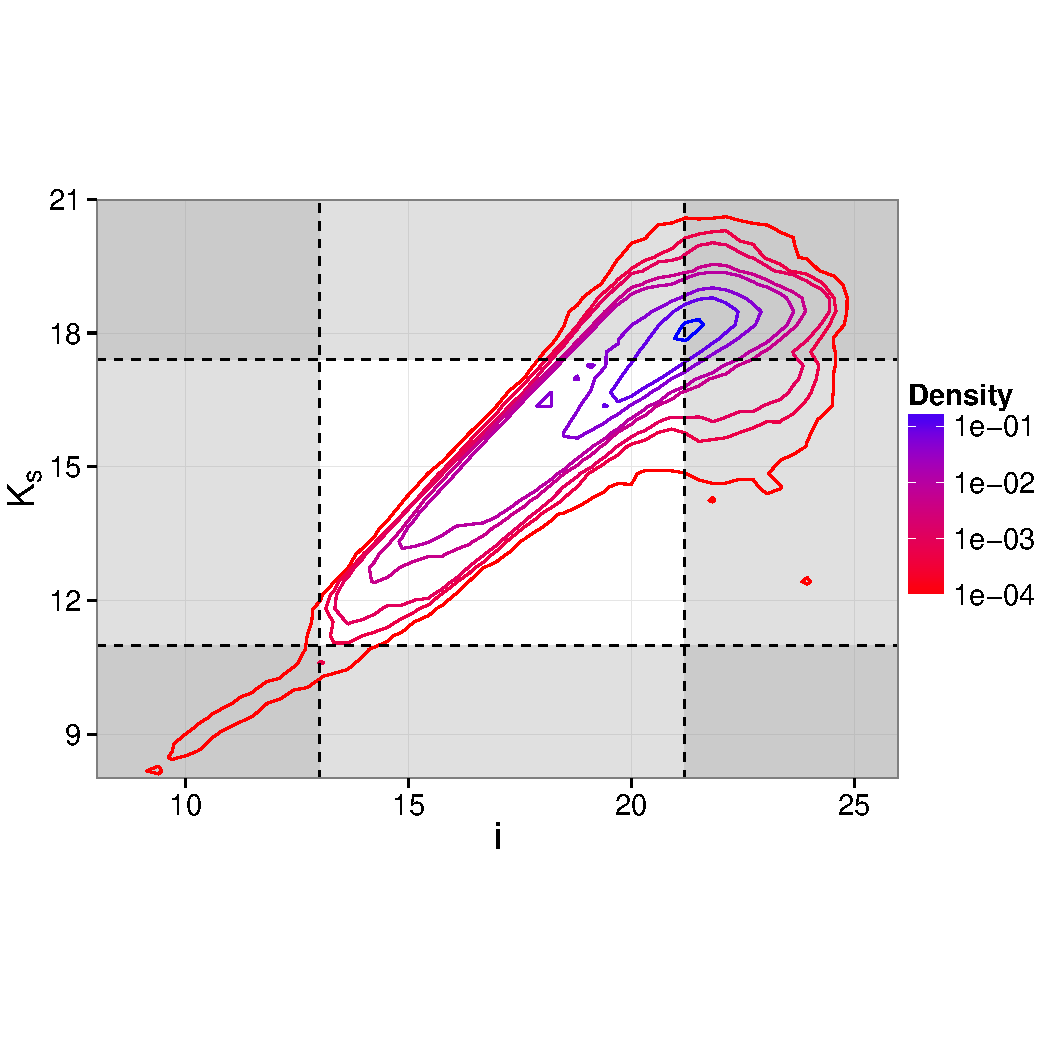
\includegraphics[width=0.8\textwidth]{background/Figures/Density-Kvsi.pdf}}
%\caption{Density of all \gls{ddr2} sources in $K_s$ and $i$ magnitudes. Lines show the chosen completeness limits, $13<i<21.2$ mag.,and $11<K_s<17.4$ mag. The grey area is considered incomplete. Reproduced from Figure 9 of \citet{Olivares2017},\textit{\usebibentry{Olivares2017}{Title}}, \usebibentry{Olivares2017}{Journal}, Vol. \usebibentry{Olivares2017}{Volume}.}
%\label{fig:completenessK+i}.
%\end{center}
%\end{figure}

In terms of proper motions, given that no selection has been performed based on these quantities, and that I assume independence between proper motions and photometry\footnote{During the summer of 2017, I co-supervised the stage of a master student who investigated the validity of this assumption. Briefly, he found only a mild correlation between the proper motions and the photometry. Once the proper motions are transformed to galactic coordinates the correlation is only present, but still negligible, along the galactic plane.}, I take it for granted that the survey is complete within the limits $|\mu_{\alpha}|,|\mu_{\delta}| < 100$ mas yr$^{-1}$ imposed by the authors of the catalogue. Nevertheless, as we will see in Section \ref{sect:field_population}, the field model accounts for this truncation.

As mentioned in Section \ref{sect:RF-2}, we will independently analyse the cluster \gls{psd} and the kinematic and photometric distributions. Nevertheless, here I gauge possible photometric incompletenesses caused by the spatial coverage of the \gls{ddr2} data. To do it I assume that the true population of sources in the sky area covered by the \gls{ddr2} is homogeneously distributed. This is a simplistic assumption that discards inhomogeneities introduced by the cluster and the galaxy. Nevertheless, it suffices to roughly quantify the completeness. Figure \ref{fig:sptph_completeness} shows the spatial completeness, in each photometric band, as a function of the maximum magnitude of the sources contained within the given limiting radius. The latter is measured from the cluster centre \cite[R.A. = 56.65$^\circ$, Dec. = 24.13$^\circ$][]{Bouy2015}. The completeness is measured as the ratio of the observed to expected density of sources, where the expected density is computed from two million synthetic sources uniformly distributed within a radius of 6$^\circ$. As can be seen from this Figure, the spatial and photometric completeness of the $Y,J,H$ and $K_s$ bands drops near the limits imposed by the sky coverage and limiting magnitudes of \gls{ukidss}. However, the $i$ band is only partially complete. The latter arise due to the different spatial coverage and limiting magnitudes of the \gls{apass} and CFHT/MegaCam date sets.

\begin{figure}[ht!]
\begin{center}
    \begin{subfigure}[t]{0.49\textwidth}
        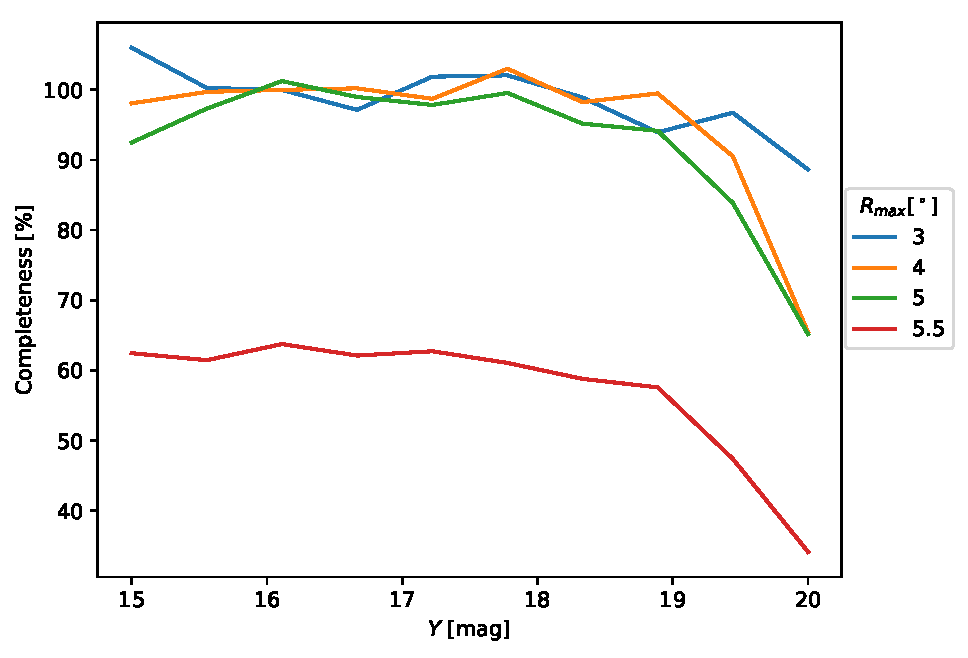
\includegraphics[page=1,height=6cm,width=8cm]{background/Figures/PhotoSpatialCompleteness_PDDR2.pdf}
    \end{subfigure}
    \begin{subfigure}[t]{0.49\textwidth}
      \includegraphics[page=2,height=6cm,width=8cm]{background/Figures/PhotoSpatialCompleteness_PDDR2.pdf}
    \end{subfigure}
     \begin{subfigure}[t]{0.49\textwidth}
      \includegraphics[page=3,height=6cm,width=8cm]{background/Figures/PhotoSpatialCompleteness_PDDR2.pdf}
    \end{subfigure}
     \begin{subfigure}[t]{0.49\textwidth}
      \includegraphics[page=4,height=6cm,width=8cm]{background/Figures/PhotoSpatialCompleteness_PDDR2.pdf}
    \end{subfigure}
    \begin{subfigure}[t]{0.49\textwidth}
      \includegraphics[page=5,height=6cm,width=8cm]{background/Figures/PhotoSpatialCompleteness_PDDR2.pdf}
    \end{subfigure}
\end{center}    
\caption{Spatial and photometric completeness of the \gls{ddr2} as a function of limiting magnitude and maximum radius of sky coverage.}
\label{fig:sptph_completeness}
\end{figure}


\subsection{Missing values}
\label{sect:ddr2_missing}

As can be verified from Table \ref{tab:DR2properties}, the amount of \gls{ddr2} sources with missing values is not negligible.  
However, objects with at least one observable marked as a missing value\footnote{Usually marked as Not Available (NA) or Not A Number (NAN).} occur only in the photometric measurements (see Table \ref{tab:DR2properties}), with the bluer bands being the most affected. As expected, the probability distribution of sources with missing values is not uniform. Missing values occur with higher probability at the faintest end of the photometric distributions ($\sim 18$ mag in $J,H$ and $K_s$ bands). Figure \ref{fig:NAsDDR2} shows the distribution of objects in the \gls{ddr2} (resulting after the restrictions mentioned in previous sections) having at least one missing entry in one band, as a function of the band that is actually observed. The vast majority of these objects occur at the faint end, close to the sensitivity limits of the survey, which coincide with those of the the \gls{ukidss} Galactic Cluster Survey \cite[$Y\sim 20.3$, $J\sim19.5$, $H\sim K_s\sim18.6$ according to][ and shown in Figure \ref{fig:NAsDDR2} with vertical dotted lines]{2007MNRAS.379.1599L}. In this Figure, the bumps at the bright and middle ranges arise due to the mixing of surveys. The first bump corresponds to the survey carried out by \citet{Bouy2015}. As mentioned in their Appendix A, due to saturation, the $Y$ band photometry was limited to objects fainter than $\sim 13$ magnitude. Thus, they complemented the Pleiades \gls{dance} catalogue with shallow $Y$ band photometry in the magnitude range of 8 to 14 magnitudes but only for 40 candidate members of \citet{Stauffer2007} and their surrounding objects \cite[see][for more details]{Bouy2015}. Thus, the large amount of missing $Y$ values in the 8 to 14 mag range of Fig. \ref{fig:NAsDDR2} come from those objects not observed by these authors. The second bump at the middle range is slightly fainter than the sensitivity limits of the \gls{2mass} survey ($J\sim 16.4$, $H\sim15.5$ and $K_s \sim 14.8$, see Section 6.2 of the Explanatory Supplement to the \gls{2mass} All Sky Data Release\footnote{\url{https://www.ipac.caltech.edu/2mass/releases/allsky/doc/sec6_2.html}}), which indicates that it comes from the mixing of the \gls{2mass} and \gls{ukidss} surveys. Due to the different spatial resolutions, some objects are detected in \gls{2mass} and not in \gls{ukidss} (e.g. pairs that are resolved in the former but unresolved in the latter).

\begin{figure}[ht!]
    \centering
    \begin{subfigure}[t]{0.45\textwidth}
        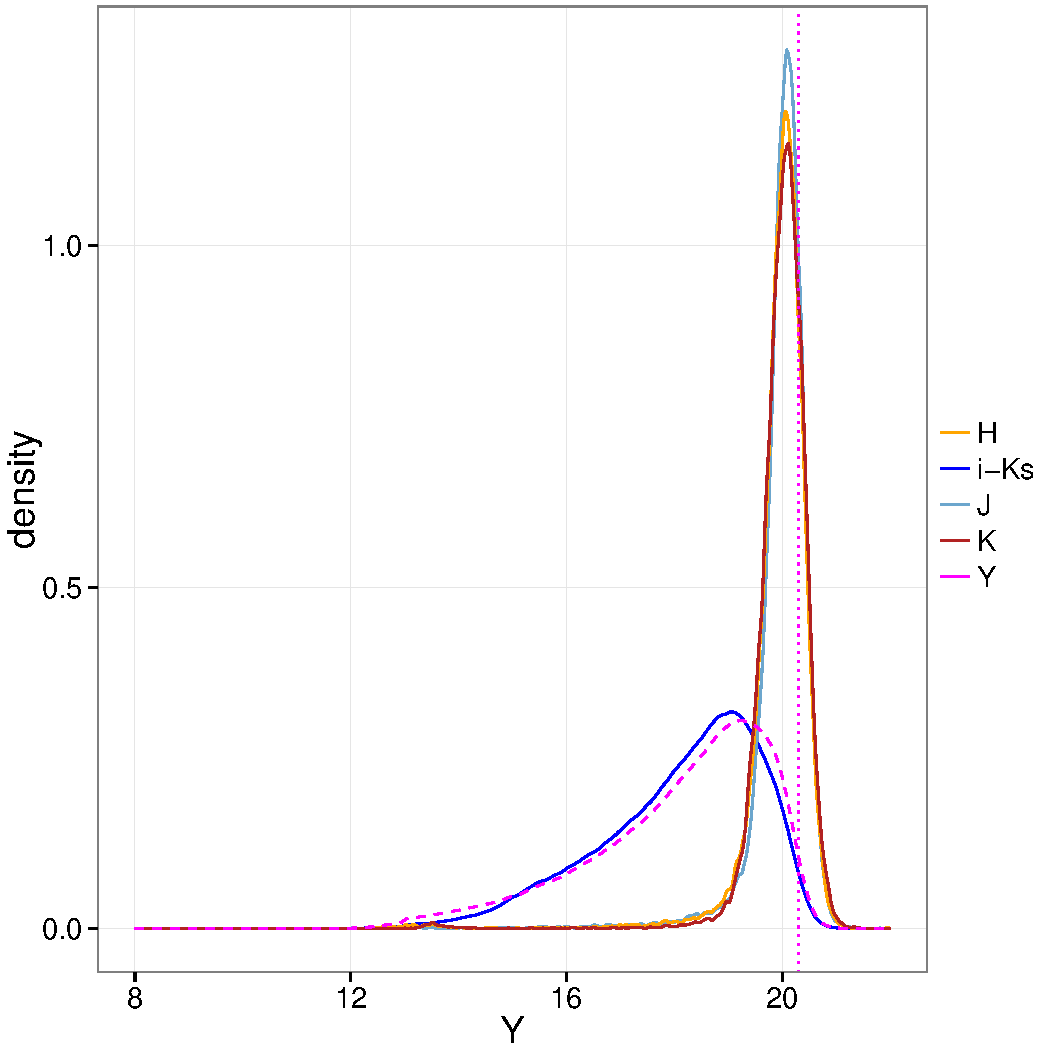
\includegraphics[page=1,height=7cm]{background/Figures/MissingDistributionsDDR2.pdf}
    \end{subfigure}
    \begin{subfigure}[t]{0.45\textwidth}
      \includegraphics[page=2,height=7cm]{background/Figures/MissingDistributionsDDR2.pdf}
    \end{subfigure}
     \begin{subfigure}[t]{0.45\textwidth}
      \includegraphics[page=3,height=7cm]{background/Figures/MissingDistributionsDDR2.pdf}
    \end{subfigure}
     \begin{subfigure}[t]{0.45\textwidth}
      \includegraphics[page=4,height=7cm]{background/Figures/MissingDistributionsDDR2.pdf}
    \end{subfigure}
\caption{Density distributions in $Y,J,H$ and $K_s$ bands for \gls{ddr2} objects with missing values in the other bands. For comparison, the distribution of observed objects is also shown with a dashed line. The majority of the missing value objects are located at the faint end of the magnitude distributions, which roughly correspond to the sensitivity limits of \gls{ukidss}: $Y \sim 20$, $J \sim 19$, $H\sim18.5$, and $K_s \sim 18$, which are marked by vertical dotted lines. A non negligible fraction of missing  $Y$ band photometry is at the bright end ($J,H,K_s \sim 8 - 14$ mag), and in the middle range of 13 to 16 magnitudes. See text for details.}
\label{fig:NAsDDR2}
\end{figure}


\section{The Restricted DANCe Data Release 2 (RDDR2)}
\label{sect:RDR2}

As I will show in Section \ref{sect:BHM}, the methodology developed in this work is computationally demanding. This, in addition to our computational constraints (see Section \ref{sect:HHPC}), prevented us to apply it in the entire \gls{ddr2} described in the previous sections.
However, the precision of our methodology, as that of any statistical analysis, increases with the number of independent observations. Therefore, we are forced to find a balance between sample size and computing time spent on analysing it. Proceeding in an heuristic way, we find that a size of $10^5$, which nevertheless takes four weeks to be analysed (see Section \ref{sect:code} for details on the computing facilities), represents a reasonable compromise between size and computing time.

Although a smaller data set produces faster results (within days), it also renders a less precise and potentially more biased model of the field. The latter results in a more contaminated model of the cluster. To restrict the size of the data set we decided to select objects based on its membership probability to the cluster. This decision is based upon the following premises.

\begin{itemize}
\item Our main objective is to characterise the cluster population. 
\item Computational time is expensive and limited.
\end{itemize}
 
By selecting objects based on membership probability, we ensure ourselves to avoid expending expensive and limited computing time in objects that most likely belong to the field, and thus fall outside our objective. Thus, we restrict the\gls{ddr2} to the $10^5$ objects with highest membership probabilities according to \citet{Bouy2015}. This selection is equivalent to set a probability threshold at membership probability of $p=1.05 \times 10^{-11}$. In the following I will refer to this data set as the \gls{rdr2}. Performing this selection has two important consequences.

Since the field objects within the \gls{rdr2} are no longer a representative sample of the field population, the field model should be constructed using this sample.

Since the probability of leaving a cluster member out of the \gls{rdr2} is less than $p=1.05 \times 10^{-11}$, we can safely assume that the completeness limits of the \gls{ddr2} (estimated in Section \ref{sect:ddr2_completeness}) apply to the cluster population present in the \gls{rdr2}, and only to it. This selection of objects depends deeply on the membership probabilities estimated by \citet{Bouy2015}. However, the large size of the \gls{rdr2} data set ($10^5$), compared to the cluster population ($\sim2000$), and the lower value of the membership probability threshold ($p=1.05 \times 10^{-11}$), ensure that leaving out a true cluster members is highly unlikely. This assumption will be corroborated in Section \ref{sect:memberscomparison}, where membership probabilities for all the objects in the \gls{ddr2} are estimated \emph{a posteriori}, once the cluster model is learnt from the \gls{rdr2}. Here, I anticipate that no cluster member is found outside the \gls{rdr2}, which confirm this assumption.

Tables \ref{tab:rddr2_cluster} and \ref{tab:rddr2_field} show summaries of the observables and uncertainties for the 98012 field and 1988 cluster objects in the \gls{rdr2}, respectively. This classification is based on the membership probabilities and probability threshold ($p=0.75$) derived by \citet{Bouy2015}.

\begin{table}[ht!]
\caption{Summary of the 1988 candidate members of \citet{Bouy2015} in the \gls{ddr2}.}
\begin{center}
\begin{tabular}{|c|c|c|c|c|c|c|c|}
\hline
Observable & Min. & 1st. Qu. & Median & Mean & 3rd. Qu. & Max. & NA's \\
\hline
\hline
$\mu_{\alpha} [mas\cdot yr^{-1}]$&-81.64 &  14.45  & 16.24 &  16.30  & 18.14  & 90.32&0\\
$\mu_{\delta} [mas\cdot yr^{-1}]$&-81.88&  -42.09 & -39.85  & -39.62  &-37.45  & 82.59&0\\
i -$K_s$[mag] &  0.934 &   3.002 &  3.364  & 3.396 &  3.678 &  7.085  &   713\\
Y [mag]& 8.284 & 13.700 & 14.450  &14.690  &15.400 & 20.390  &   518\\
J [mag]& 6.545 & 11.950 & 13.400  &13.160 & 14.380  &19.310   &    6\\
H [mag]& 6.587 & 11.330 & 12.850  &12.610&  13.840 & 18.300   &   13\\
$K_s$ [mag]& 6.514 & 11.090 & 12.530 & 12.300 & 13.500 & 17.360   &    1\\
\hline
\multicolumn{8}{c}{Uncertainties}\\
\hline
Observable & Min. & 1st. Qu. & Median &Mean& 3rd. Qu. & Max. & NA's \\
\hline
\hline
$\mu_{\alpha} [mas\cdot yr^{-1}]$&0.08&0.25&0.76&0.5201&2.02&1e+5 &0\\ 
$\mu_{\delta} [mas\cdot yr^{-1}]$&0.08&0.25&0.76&0.52&2.02&1e+5& 0\\ 
i [mag] & 0.0200 & 0.0200 & 0.0200 & 0.0351 & 0.0202 & 2.1610&713 \\
Y [mag] & 0.0300&  0.0500&  0.0501&  0.0569&  0.0503 & 0.2392&518\\
J [mag] & 0.02000& 0.02700& 0.05005 &0.04270& 0.05014 &0.15990&6\\
H [mag] & 0.02000 &0.02700& 0.04009 &0.03994 &0.05010 & 0.14340&13\\
$K_s$[mag]&0.02000& 0.05003& 0.05045& 0.05278 &0.06001 &9.99500&1\\
\hline
\end{tabular}
\end{center}
\label{tab:rddr2_cluster}
\end{table}%

\begin{table}[ht!]
\caption{Summary of the 98012 filed objects in the \gls{rdr2}.}
\begin{center}
\begin{tabular}{|c|c|c|c|c|c|c|c|}
\hline
Observable & Min. & 1st. Qu. & Median & Mean & 3rd. Qu. & Max. & NA's \\
\hline
\hline
$\mu_{\alpha} [mas\cdot yr^{-1}]$&-99.980& -11.730  & 1.803 &  1.307 & 15.050 & 99.910&0\\
$\mu_{\delta} [mas\cdot yr^{-1}]$&-99.990& -17.980  &-4.820  &-4.088   &9.189  &99.980&0\\
i -$K_s$[mag] &   1.04 &   3.49  &  5.13    &   4.81  &  5.81  &  7.99 &  95628 \\
Y [mag]          & 9.97  & 18.70      &  19.45 &  18.83 &  19.93 &  22.23  & 21988 \\
J [mag]          & 3.954 & 17.790 & 18.660 & 17.880 & 19.160 & 20.620 &   7305\\
H [mag]         & 2.969 & 16.950 & 17.750 & 17.020 & 18.210 & 20.270  &  7655\\
$K_s$ [mag] & 2.598 & 16.260 & 16.960  &16.360  &17.370 & 21.020 &   5013\\
\hline
\multicolumn{8}{c}{Uncertainties}\\
\hline
Observable & Min. & 1st. Qu. & Median &Mean& 3rd. Qu. & Max. & NA's \\
\hline
\hline
$\mu_{\alpha} [mas\cdot yr^{-1}]$&0.08  &    8.65   &  14.94   &  23.50   &  25.60 &1.0e+05&0\\ 
$\mu_{\delta} [mas\cdot yr^{-1}]$&0.085  &   8.652  &  14.940  &  20.710  &  25.600 &1.86e+04 & 0\\ 
i [mag] & 0.02        &  0.02    &    0.07 &   0.08 &  0.12   & 0.66    &    95628 \\
Y [mag] & 0.030     &   0.068&   0.103&  0.112 &   0.148&0.938  &   21988\\
J [mag] & 0.020      &  0.065  & 0.097  & 0.104 & 0.136  &0.403   & 7305\\
H [mag] & 0.020     &  0.065  & 0.093  &0.099  & 0.124  &9.998   & 7655\\
$K_s$[mag]&0.020 &  0.060 &  0.079 & 0.087  & 0.101 & 9.998  & 5013\\
\hline
\end{tabular}
\end{center}
\label{tab:rddr2_field}
\end{table}%

\subsection{Missing values}

Since the \gls{rdr2} is not a random sample of the \gls{ddr2}, the distributions of objects containing missing values are not the same as those shown in Section \ref{sect:ddr2_missing}. Thus, Fig. \ref{fig:NAs} shows the distribution of objects containing missing entries in one band as a function of magnitude in the other bands. 

\begin{figure}[ht!]
    \centering
    \begin{subfigure}[t]{0.45\textwidth}
        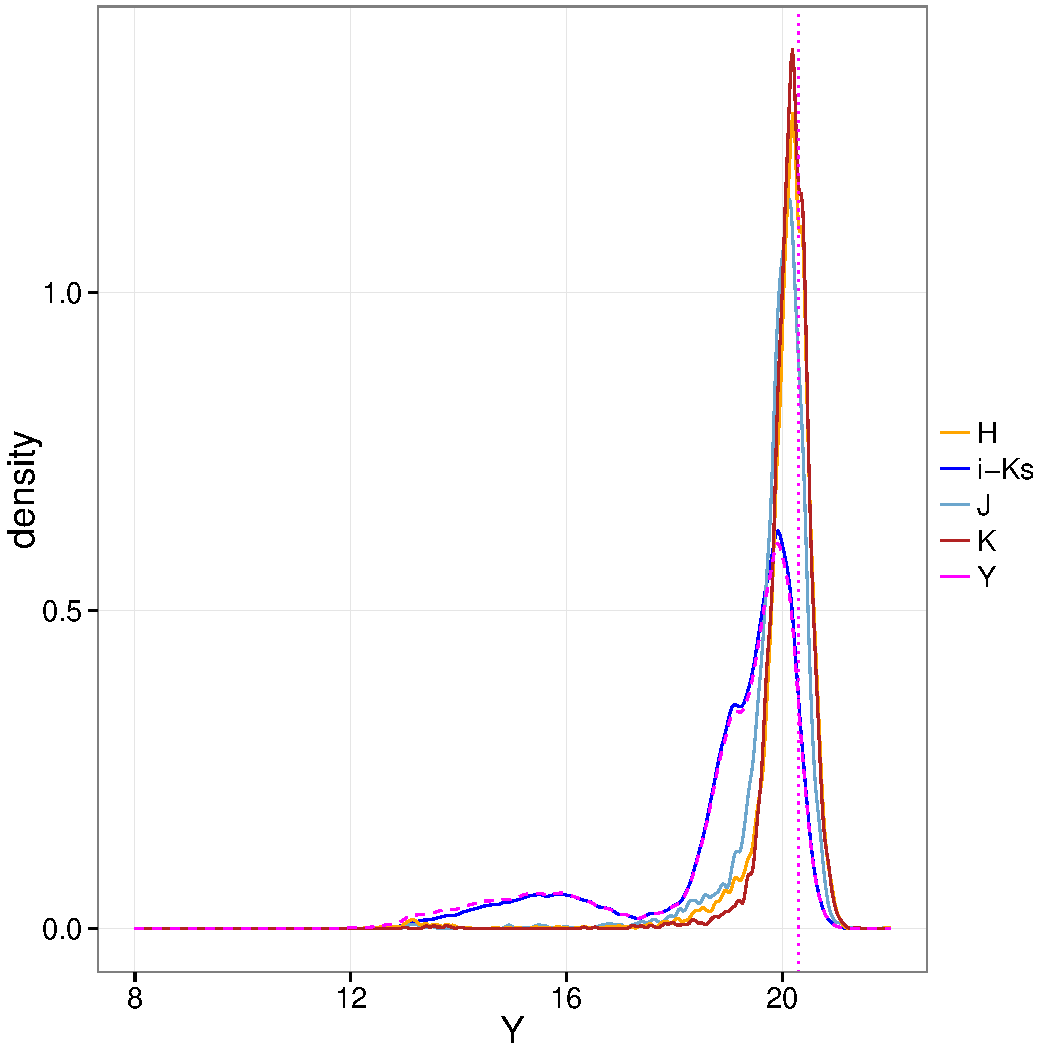
\includegraphics[page=1,height=7cm]{background/Figures/MissingDistributions.pdf}
    \end{subfigure}
    \begin{subfigure}[t]{0.45\textwidth}
      \includegraphics[page=2,height=7cm]{background/Figures/MissingDistributions.pdf}
    \end{subfigure}
     \begin{subfigure}[t]{0.45\textwidth}
      \includegraphics[page=3,height=7cm]{background/Figures/MissingDistributions.pdf}
    \end{subfigure}
     \begin{subfigure}[t]{0.45\textwidth}
      \includegraphics[page=4,height=7cm]{background/Figures/MissingDistributions.pdf}
    \end{subfigure}
\caption{Density distributions in $Y,J,H$ and $K_s$ bands of \gls{rdr2} for objects with missing values in the other bands. For comparison, the distribution of observed objects is also shown with a dashed line. The features are similar to those in Fig. \ref{fig:NAsDDR2}. The small differences between the two figures come from the fact that the \gls{rdr2} is not a random sample of the \gls{ddr2}.}
\label{fig:NAs}
\end{figure}

In addition, Fig \ref{fig:mis_vs_obs} shows the magnitude distributions of completely observed objects (without missing values) compared to those of all objects, including those with missing entries. This Figure shows that the distributions of objects with completely observed photometry is highly discrepant from that of the entire population. Thus probing that our analysis can not be based only on objects with completely observed photometry, and that the treatment of missing values is of paramount importance (more details will be given in Section \ref{sect:missing}).

\begin{figure}[ht!]
    \centering
      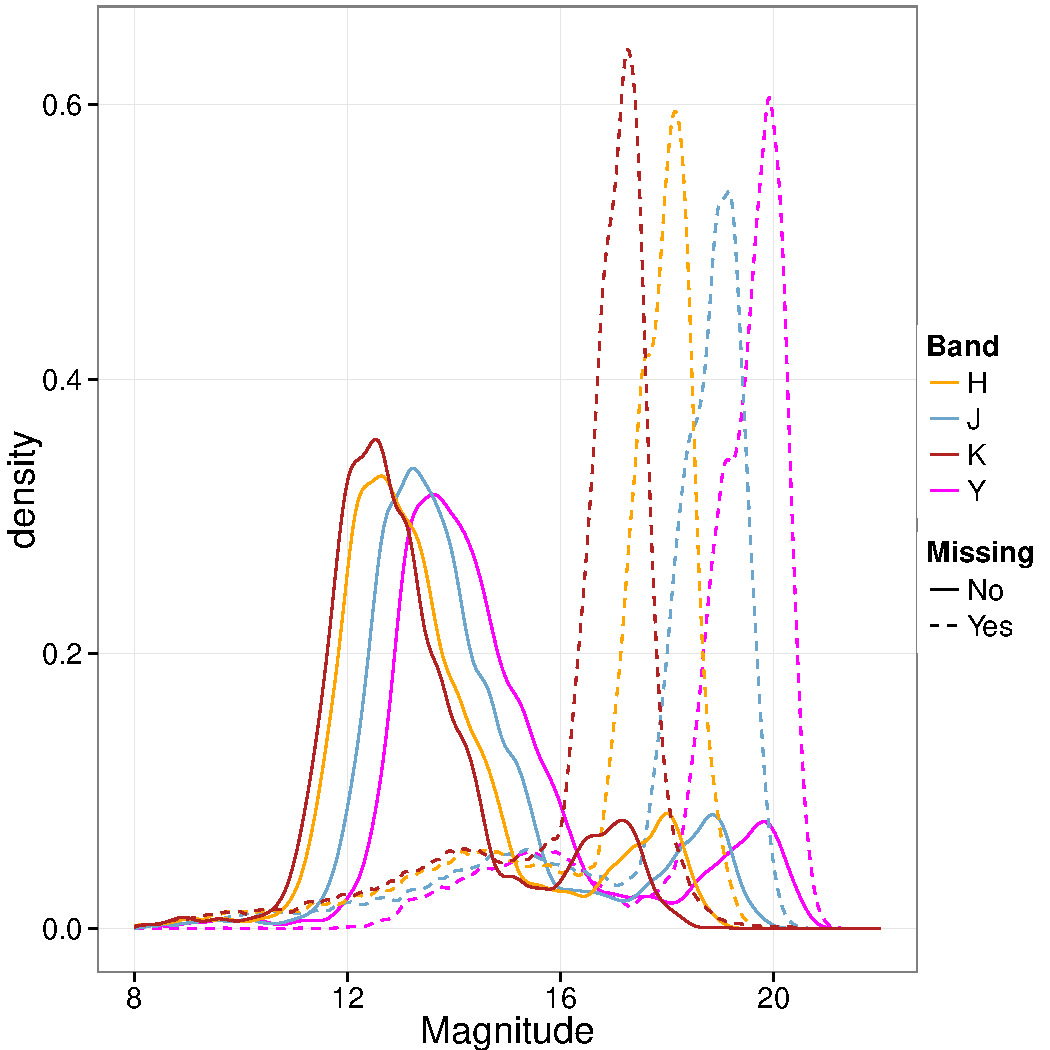
\includegraphics[page=1,width=0.8\textwidth]{background/Figures/ObservedDistributions.pdf}
\caption{Density distributions in $Y,J,H$ and $K_s$ bands of \gls{rdr2} for objects with: a) at least one missing entry (dashed lines), and b) no-missing entries (solid line).}
\label{fig:mis_vs_obs}
\end{figure}



\section{The Tycho+DANCe candidate members}
\label{sect:Tycho+DANCe}

As mentioned in Section \ref{sect:RF-2}, we will independently analyse the cluster \gls{psd} and the kinematic and photometric distributions.
Thus, here I describe the data set used for the analysis of the Pleiades \gls{psd}. It comprises, for the middle and faint luminosities, the \gls{hmps} of candidate members recovered by the \gls{bhm}, described in Section \ref{sect:memberscomparison}, and summarised in Table \ref{tab:hmps}, and for the high luminosities, the Tycho+DANCe candidate members of \cite{Bouy2015}, summarised in Table \ref{tab:tycho2}. This data set is the largest and less contaminated list of Pleiades candidate members to date. 

This joint data set contains the positions, in equatorial coordinates R.A. and Dec. (in the following $\alpha$ and $\delta$), proper motions, photometry, and membership probabilities of 2060 unique candidate members. For the analysis of the \gls{psd} we work only with the positions, membership probabilities, and $J$ photometric band. The latter is the bluest most available photometric band for this list of members. It will be used as a proxy for the mass, and to explore evidence of mass segregation.

\begin{table}[ht!]
\caption{Summary of the 1967 objects classified as members by the \gls{bhm}.}
\begin{center}
\begin{tabular}{|c|c|c|c|c|c|c|c|}
\hline
Observable & Min. & 1st. Qu. & Median & Mean & 3rd. Qu. & Max. & NA's \\
\hline
\hline
RA [deg]   & 51.42 &  55.67 & 56.69 &  56.76  & 57.81  & 62.81 & 0\\
Dec. [deg] &19.13  & 23.11  & 24.10 &  24.13  & 25.22 &  29.56 &0\\
$\mu_{\alpha} [mas\cdot yr^{-1}]$&-23.34  & 14.59  & 16.32 &  16.73 &  18.37  & 53.84&0\\
$\mu_{\delta} [mas\cdot yr^{-1}]$&-81.370 &-42.410& -40.130& -40.480& -37.760&  -2.016&0\\
i -$K_s$[mag] &  0.934 &  2.979  & 3.357    & 3.325   &  3.648  &6.662   &643\\
Y [mag]           &   8.284 & 13.660 & 14.360  &14.590  &15.310  &20.100 &   467 \\
J [mag]           &   7.058 & 12.060& 13.370  & 13.180 & 14.290 & 18.570&      5\\
H [mag]          &   7.009 & 11.430 & 12.810  & 12.620 & 13.750 & 17.480&      9 \\
$K_s$ [mag]  &   7.008 & 11.190 & 12.500  & 12.320 & 13.410 & 16.740&    0\\
\hline
\end{tabular}
\end{center}
\label{tab:hmps}
\end{table}%

\begin{table}[ht!]
\caption{Summary of the 207 objects from the Tycho2+DANCe data set classified as Pleiades candidate members ($P>0.48)$ by \citet{Bouy2015}.}
\begin{center}
\begin{tabular}{|c|c|c|c|c|c|c|c|}
\hline
Observable & Min. & 1st. Qu. & Median & Mean & 3rd. Qu. & Max. & NA's \\
\hline
\hline
RA [$^\circ$]                                 				            &  52.05&55.89 & 56.46 &56.55  &57.30   &  62.49  & 0\\
Dec. [$^\circ$]                       					           &  18.56&23.13  & 24.08& 23.99  &24.88  & 29.89 &0\\
$\mu_{\alpha} [\mathrm{mas}\cdot \mathrm{yr}^{-1}]$   &      9.7 &18.9   & 20.1  &    20.0 &  21.1   &  26.7&0\\
$\mu_{\delta} [\mathrm{mas}\cdot \mathrm{yr}^{-1}]]$   &  -55.10&-46.60&-45.10&-45.19 &-43.70  & -37.70&0\\
i [mag]								            &   7.910&9.321 & 10.21&  10.04 &   10.76& 12.960&   72\\
J [mag]          								    &   3.800& 7.588& 8.638& 8.451 & 9.575  &10.590&      0\\
H [mag]        								    &   3.864& 7.535& 8.463& 8.236 & 9.209  & 10.030&      0 \\
$K_s$ [mag]  							            &   3.879&7.478 & 8.373& 8.167  &  9.113 &  9.929&    0\\
\hline
\end{tabular}
\end{center}
\label{tab:tycho2}
\end{table}%

\subsection{Contamination and completeness}
\label{sect:TDContamination}
In Section \ref{sect:classifier}, we estimate a contamination rate of $4.3\pm0.2$\% in the \gls{hmps}, which
would amount to 84 of the 1967 candidate members. Also, \citet{Sarro2014} estimate that the contamination rate of their methodology is $11.0\pm2.0$\% for a probability threshold of $p=0.5$, as the one used by \citet{Bouy2015} to classify the candidate members of their \gls{t+d} data set.  Thus, in our combined \gls{t+d} list of candidate members, we acknowledge a mean contamination rate of $\sim 8\%$. We would expect these contaminating sources to be uniformly distributed in right ascension and declination because the position on the sky was explicitly removed from the calculation of membership probabilities.

We estimate the completeness of our list of candidate members, in terms of the $J$ band luminosity and
spatial coverage, by assessing the completeness of the joint \gls{t+d} survey. In Fig. \ref{fig:completenessT+D} we show the distribution of the number of sources in the combined \gls{t+d} catalogue as a function of the radial position for different limiting magnitudes in the $J$ band.
The radial position is computed assuming a distance of 134.4 pc to the Pleiades cluster \citep{Galli2017} and a centre at $\alpha,\delta =[56.65,24.13]$. Distances are corrected by geometric distortions of large angles (using Eqs. \ref{eq:distfree} and \ref{eq:rs_and_ts}).
As can be seen from this figure, the \gls{t+d} catalogue is complete until magnitude $J\sim19$ and radial distance of 11.5 pc ($\sim5^\circ$). We notice that the latter corresponds roughly with the sky coverage of the \gls{ukidss} survey \citep{2007MNRAS.379.1599L}.
Hence, we restrict our list of candidate members to those with: i) $J$ band observed and less than 19 mag., and ii) radial distances less than 11.5 pc. This results in 1964 candidate members, which represents more than 50\% more candidate members that those of  \citet{Converse2010}, who did the latest analysis of the Pleiades \gls{psd}.

Nevertheless, we remind the reader that the inhomogeneities (e.g. spatial resolutions, gaps in luminosity) of the \gls{t+d} data set are so complex (and some of them only partially understood) that can indeed bias the sample of candidate members in unknown ways. For example, the gap in luminosity coverage between the faint end of Tycho-2 catalogue and the bright end of the DANCe survey (see in Fig. 8 of \citealt{Bouy2015}) may result in undetected sources, therefore unmeasured proper motions and finally an incomplete list of candidate members.

\begin{figure}[ht!]
\begin{center}
\includegraphics[page=2,width=0.8\textwidth]{./background/Figures/RadiiDistribution_Tycho+DANCe_Jmag.pdf}
\caption{Density of sources in the combined \gls{t+d} catalogue as a function of the radial distance to the cluster centre and limiting magnitude in the J band. The vertical grey line marks the limit of spatial completeness, 11.5 pc.}
\label{fig:completenessT+D}
\end{center}
\end{figure}




